\documentclass[12pt,a4paper]{report}
\usepackage[utf8]{inputenc}
\usepackage[english]{babel}
\usepackage{graphicx}
\usepackage{amsmath}
\usepackage{amssymb}
\usepackage{hyperref}
\usepackage{booktabs}
\usepackage{listings}
\usepackage{color}
\usepackage{geometry}
\usepackage{float}
\usepackage{tabularx}
\geometry{margin=2.5cm}
\usepackage{setspace}
\onehalfspacing
\setlength{\parindent}{1cm}
\setlength{\parskip}{0pt}

\definecolor{codegray}{rgb}{0.5,0.5,0.5}
\definecolor{codebg}{rgb}{0.95,0.95,0.95}
\lstdefinestyle{mystyle}{
    backgroundcolor=\color{codebg},
    basicstyle=\ttfamily\small,
    breakatwhitespace=false,
    breaklines=true,
    captionpos=b,
    keepspaces=true,
    numbers=left,
    numbersep=5pt,
    numberstyle=\tiny\color{codegray},
    showspaces=false,
    showstringspaces=false,
    showtabs=false,
    tabsize=2
}
\lstset{style=mystyle}

\begin{document}

% Title Page
\begin{titlepage}
    \begin{center}
        
\includegraphics[width=3cm]{images/YeditepeUniversityLogo.png} \\
        \vspace*{0.5cm}
        \large
        T.C. \\
        YEDITEPE UNIVERSITY \\
        FACULTY OF COMPUTER AND INFORMATION SCIENCES \\
        DEPARTMENT OF MANAGEMENT INFORMATION SYSTEMS \\
        
        \vspace*{1cm}
        
        \Huge
        \textbf{BORSANEURON: ALGORITHMIC STOCK PRICE FORECASTING AND AUTOMATED TECHNICAL PATTERN SCANNER PLATFORM} \\
        
        \vspace*{1cm}
        
        \large
        GitHub Repository: \href{https://github.com/zachariatrying/borsaneuron}{https://github.com/zachariatrying/borsaneuron} \\
        
        \vspace*{1cm}
        
        \Large
        \textbf{Bachelor's Thesis} \\
        
        \vspace*{0.5cm}
        
        \large
        Prepared by: \\
        \textbf{İbrahim Tatar} \\
        Student No: 20211314007 \\
        
        \vspace*{0.75cm}
        
        \large
        Thesis Advisor: \\
        \textbf{Assoc. Prof. Dr. Uğur Tevfik Kaplancalı} \\
        
        \vfill
        
        \large
        ISTANBUL, SPRING 2026
    \end{center}
\end{titlepage}

\pagenumbering{roman}

% Özet
\chapter*{Özet}
\addcontentsline{toc}{chapter}{Özet}
Bu çalışma, Borsa İstanbul (BIST) pay piyasalarındaki hisse senetlerinin teknik analiz göstergeleri ve fiyat örüntülerini kullanarak 5 günlük gelecek fiyat yönünü tahmin etmeyi ve klasik grafik formasyonlarını otomatik taramayı hedefleyen bütünsel bir karar destek platformu olan \textbf{BorsaNeuron}'u sunmaktadır. Çalışma kapsamında BIST genelini temsil eden tarihsel günlük veriler üzerinden 30 teknik indikatörlü bir özellik seti oluşturulmuş; çoklu doğrusal bağlantıyı önlemek adına korelasyon analizleri yapılmış ve pazar rejimleri K-Means kümeleme ile 5 farklı grupta segmentize edilerek Temel Bileşenler Analizi (PCA) ile görselleştirilmiştir.

Gelecek fiyat yönünü tahmin etmek amacıyla eğitilen K-En Yakın Komşu (K-NN), Yapay Sinir Ağları (ANN - MLPClassifier), Rastgele Orman (Random Forest) ve XGBoost modelleri arasından, Yapay Sinir Ağı \%55.68 doğruluk ve 0.6496 F1-Skoru ile en yüksek başarıyı göstermiştir. Üretim aşamasında ise dengeli duyarlılık ve kesinlik profili nedeniyle XGBoost modeli online tahmin motoru olarak seçilmiştir. Geliştirilen makine öğrenmesi modelleri Streamlit kütüphanesi kullanılarak interaktif bir web paneline dönüştürülmüştür. Bu arayüz; yfinance üzerinden canlı veri akışı sağlayan, hisselerin tarihsel başarı oranlarını (Win Rate) karar sürecine dahil eden ve TOBO, Fincan-Kulp, Flama, İkili Dip/Tepe formasyonlarını tarayabilen canlı bir platform sunmaktadır. Geliştirilen sistem Docker ile konteynerleştirilerek bulut dağıtımına hazır hale getirilmiştir.

\vspace*{1cm}
\noindent \textbf{Anahtar Kelimeler:} Veri Madenciliği, BIST Tahminlemesi, Makine Öğrenmesi, K-Means Kümeleme, Sektörel Kıyaslama, Streamlit, Teknik Formasyon Tarayıcı.

\newpage

% Abstract
\chapter*{Abstract}
\addcontentsline{toc}{chapter}{Abstract}
This study presents \textbf{BorsaNeuron}, a holistic decision support platform designed to forecast the 5-day future price direction of equities in the Borsa Istanbul (BIST) stock markets and automatically scan classical chart patterns using technical analysis indicators and price patterns. Within the scope of the study, a feature set of 30 technical indicators was constructed from historical daily data representing the BIST in general; correlation analyses were performed to prevent multicollinearity, and market regimes were segmented into 5 different groups using K-Means clustering and visualized with Principal Component Analysis (PCA).

Among the K-Nearest Neighbors (K-NN), Artificial Neural Networks (ANN - MLPClassifier), Random Forest, and XGBoost models trained to forecast the future price direction, the Artificial Neural Network achieved the highest success with 55.68\% accuracy and a 0.6496 F1-Score. In the production phase, the XGBoost model was selected as the online prediction engine due to its balanced precision-recall profile. The developed machine learning models were transformed into an interactive web dashboard using the Streamlit library. This interface provides a live platform that streams real-time data via yfinance, integrates historical win rates of stocks into the decision process, and scans Inverse H&S, Cup-and-Handle, Pennant, and Double Bottom/Top formations. The developed system was containerized using Docker, making it ready for cloud deployment.

\vspace*{1cm}
\noindent \textbf{Keywords:} Data Mining, BIST Price Forecasting, Machine Learning, K-Means Clustering, Sector Benchmarking, Streamlit, Technical Pattern Scanner.

\newpage

% Table of Contents
\tableofcontents

\newpage
\pagenumbering{arabic}

% 1. INTRODUCTION
\chapter{Introduction}

This study presents the \textbf{BorsaNeuron} platform, a holistic decision support and data analysis interface designed to forecast the 5-day future price direction of equities in the Borsa Istanbul (BIST) stock markets and automatically scan classical chart patterns using technical analysis indicators and machine learning algorithms.

Applying quantitative finance and data mining principles, a historical database of active BIST equities was used. The data pipelines cleaned missing data and performed Pearson correlation analysis to prevent multicollinearity exceeding the $0.90$ threshold. To capture market regimes, the K-Means algorithm divided indicator states into 5 unique clusters, which were projected into a 2D space using PCA (where PC1 and PC2 explain 52.25\% of the total variance).

To predict the 5-day price direction target (\texttt{Target\_T5}), K-NN, ANN (MLPClassifier), and Random Forest (RF) models were optimized. The ANN model achieved the highest predictive accuracy on test data with a 55.68\% accuracy rate and a 0.6496 F1-Score. In the production dataset expanded until June 2026, the XGBoost Classifier was deployed as the online prediction engine due to its balanced precision-recall profile.

To transform the modeling pipelines into a live business intelligence tool, an interactive web panel (BorsaNeuron Dashboard) was built using the Streamlit library. The platform allows users to query BIST tickers, generate predictions using live yfinance data, adjust risk thresholds based on the stock's win rate, and scan geometric formations such as Inverse H&S, H&S, Cup-and-Handle, Pennant, Double Bottom, and Double Top. To circumvent GitHub's 100MB upload limit, the 318MB raw dataset was compressed to 50.1MB using the LZMA (xz) algorithm and is decompressed dynamically in-memory in under 6 seconds at system startup.

% 2. PROJECT SETUP
\chapter{Project Setup}

To run the project and replicate the model development processes on your local computer, a suitable data mining and programming environment must first be set up. These tools provide us with a stable terminal to run data preprocessing scripts, train models, and deploy the web dashboard. Following the installation steps, package installations will be executed via the terminal.

\section{Prerequisite Software}
To ensure system stability and cross-platform compatibility, BorsaNeuron is based on standard software environments:
\begin{itemize}
    \item \textbf{Python v3.9 or v3.11:} Preferred due to the maturity of data mining libraries and the stability of Streamlit interface components.
    \item \textbf{Visual Studio Code (VS Code) IDE:} Used as the main development environment for code development, package debugging, and running local tests.
    \item \textbf{Git Version Control System:} Installed for code versioning, local commit processes, and synchronization with the remote GitHub repository.
\end{itemize}

\newpage
\section{Initial Setup Packages of the Project}
To prevent version conflicts of the libraries, an isolated virtual environment was created. Dependencies are defined in the \texttt{requirements.txt} file. For configuring the virtual environment and installing the libraries, the following terminal commands were executed in order:

\begin{lstlisting}[language=bash, caption=Virtual Environment Setup Steps]
# Creating virtual environment
python -m venv borsaneuron_env

# Activating virtual environment (For Windows PowerShell)
.\borsaneuron_env\Scripts\Activate.ps1

# Upgrading pip package manager
python -m pip install --upgrade pip

# Installing project libraries
pip install -r requirements.txt
\end{lstlisting}

% 3. CONSTRUCTION OF THE BORSANEURON PLATFORM AND MODULES
\chapter{Construction of the BorsaNeuron Platform and Modules}

\section{Quantitative Data Pipeline}

\subsection{Pearson Correlation Filtering}
Technical indicators generated from price series naturally exhibit a high level of multicollinearity. For example, short-term and long-term moving averages (\texttt{SMA\_20} and \texttt{EMA\_12}) move highly in parallel. This situation distorts the variance of independent variables in the dataset, leading to unstable estimation coefficients and overfitting in K-NN or linear-based models.

To solve this problem, a Pearson Correlation Matrix was created among all 30 technical indicators in the dataset. Variable pairs with correlation coefficients exceeding the $0.90$ threshold were identified:
\begin{equation}
|r_{ij}| > 0.90
\end{equation}
Highly correlated variables that repeat each other were eliminated through the created upper triangular matrix filter. Thus, while the dimensional complexity of the dataset was reduced, it was ensured that our models receive clean and independent signals.

\begin{figure}[H]
    \centering
    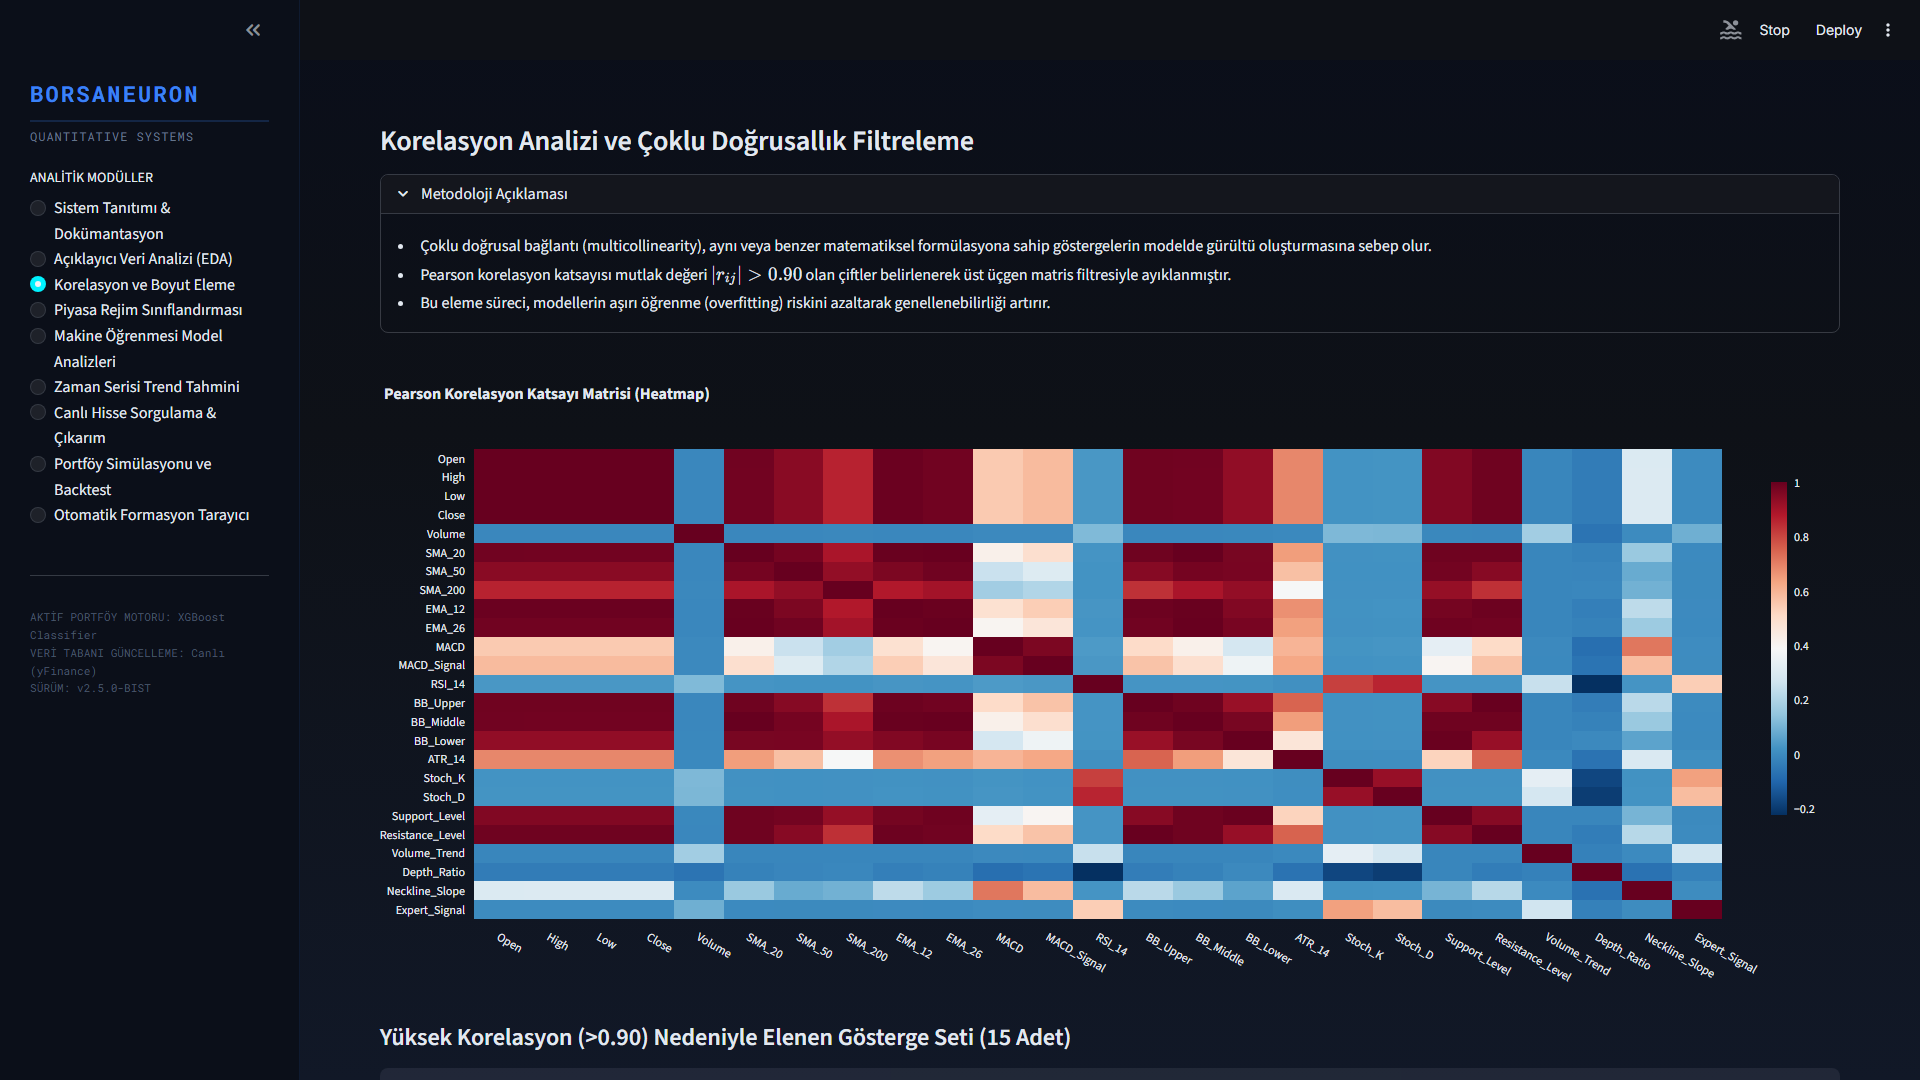
\includegraphics[width=0.85\textwidth]{images/04_korelasyon_heatmap.png}
    \caption{Heatmap showing Pearson correlation levels among technical indicators.}
    \label{fig:corr}
\end{figure}

\subsection{K-Means Market Segmentation}
Within the scope of unsupervised learning methodology, K-Means algorithm was applied to cluster market regimes according to the technical indicator states of stocks. Normalization of the data was ensured prior to clustering:
\begin{equation}
z = \frac{x - \mu}{\sigma}
\end{equation}
Elbow analysis was performed to mathematically validate the optimum number of clusters. As the number of clusters increased, the rate of decrease in the within-cluster sum of squared errors (inertia) was examined, and \textbf{$k=5$}, which is the elbow point where the inertia curve bends, was selected as the optimum number of clusters.

\begin{figure}[H]
    \centering
    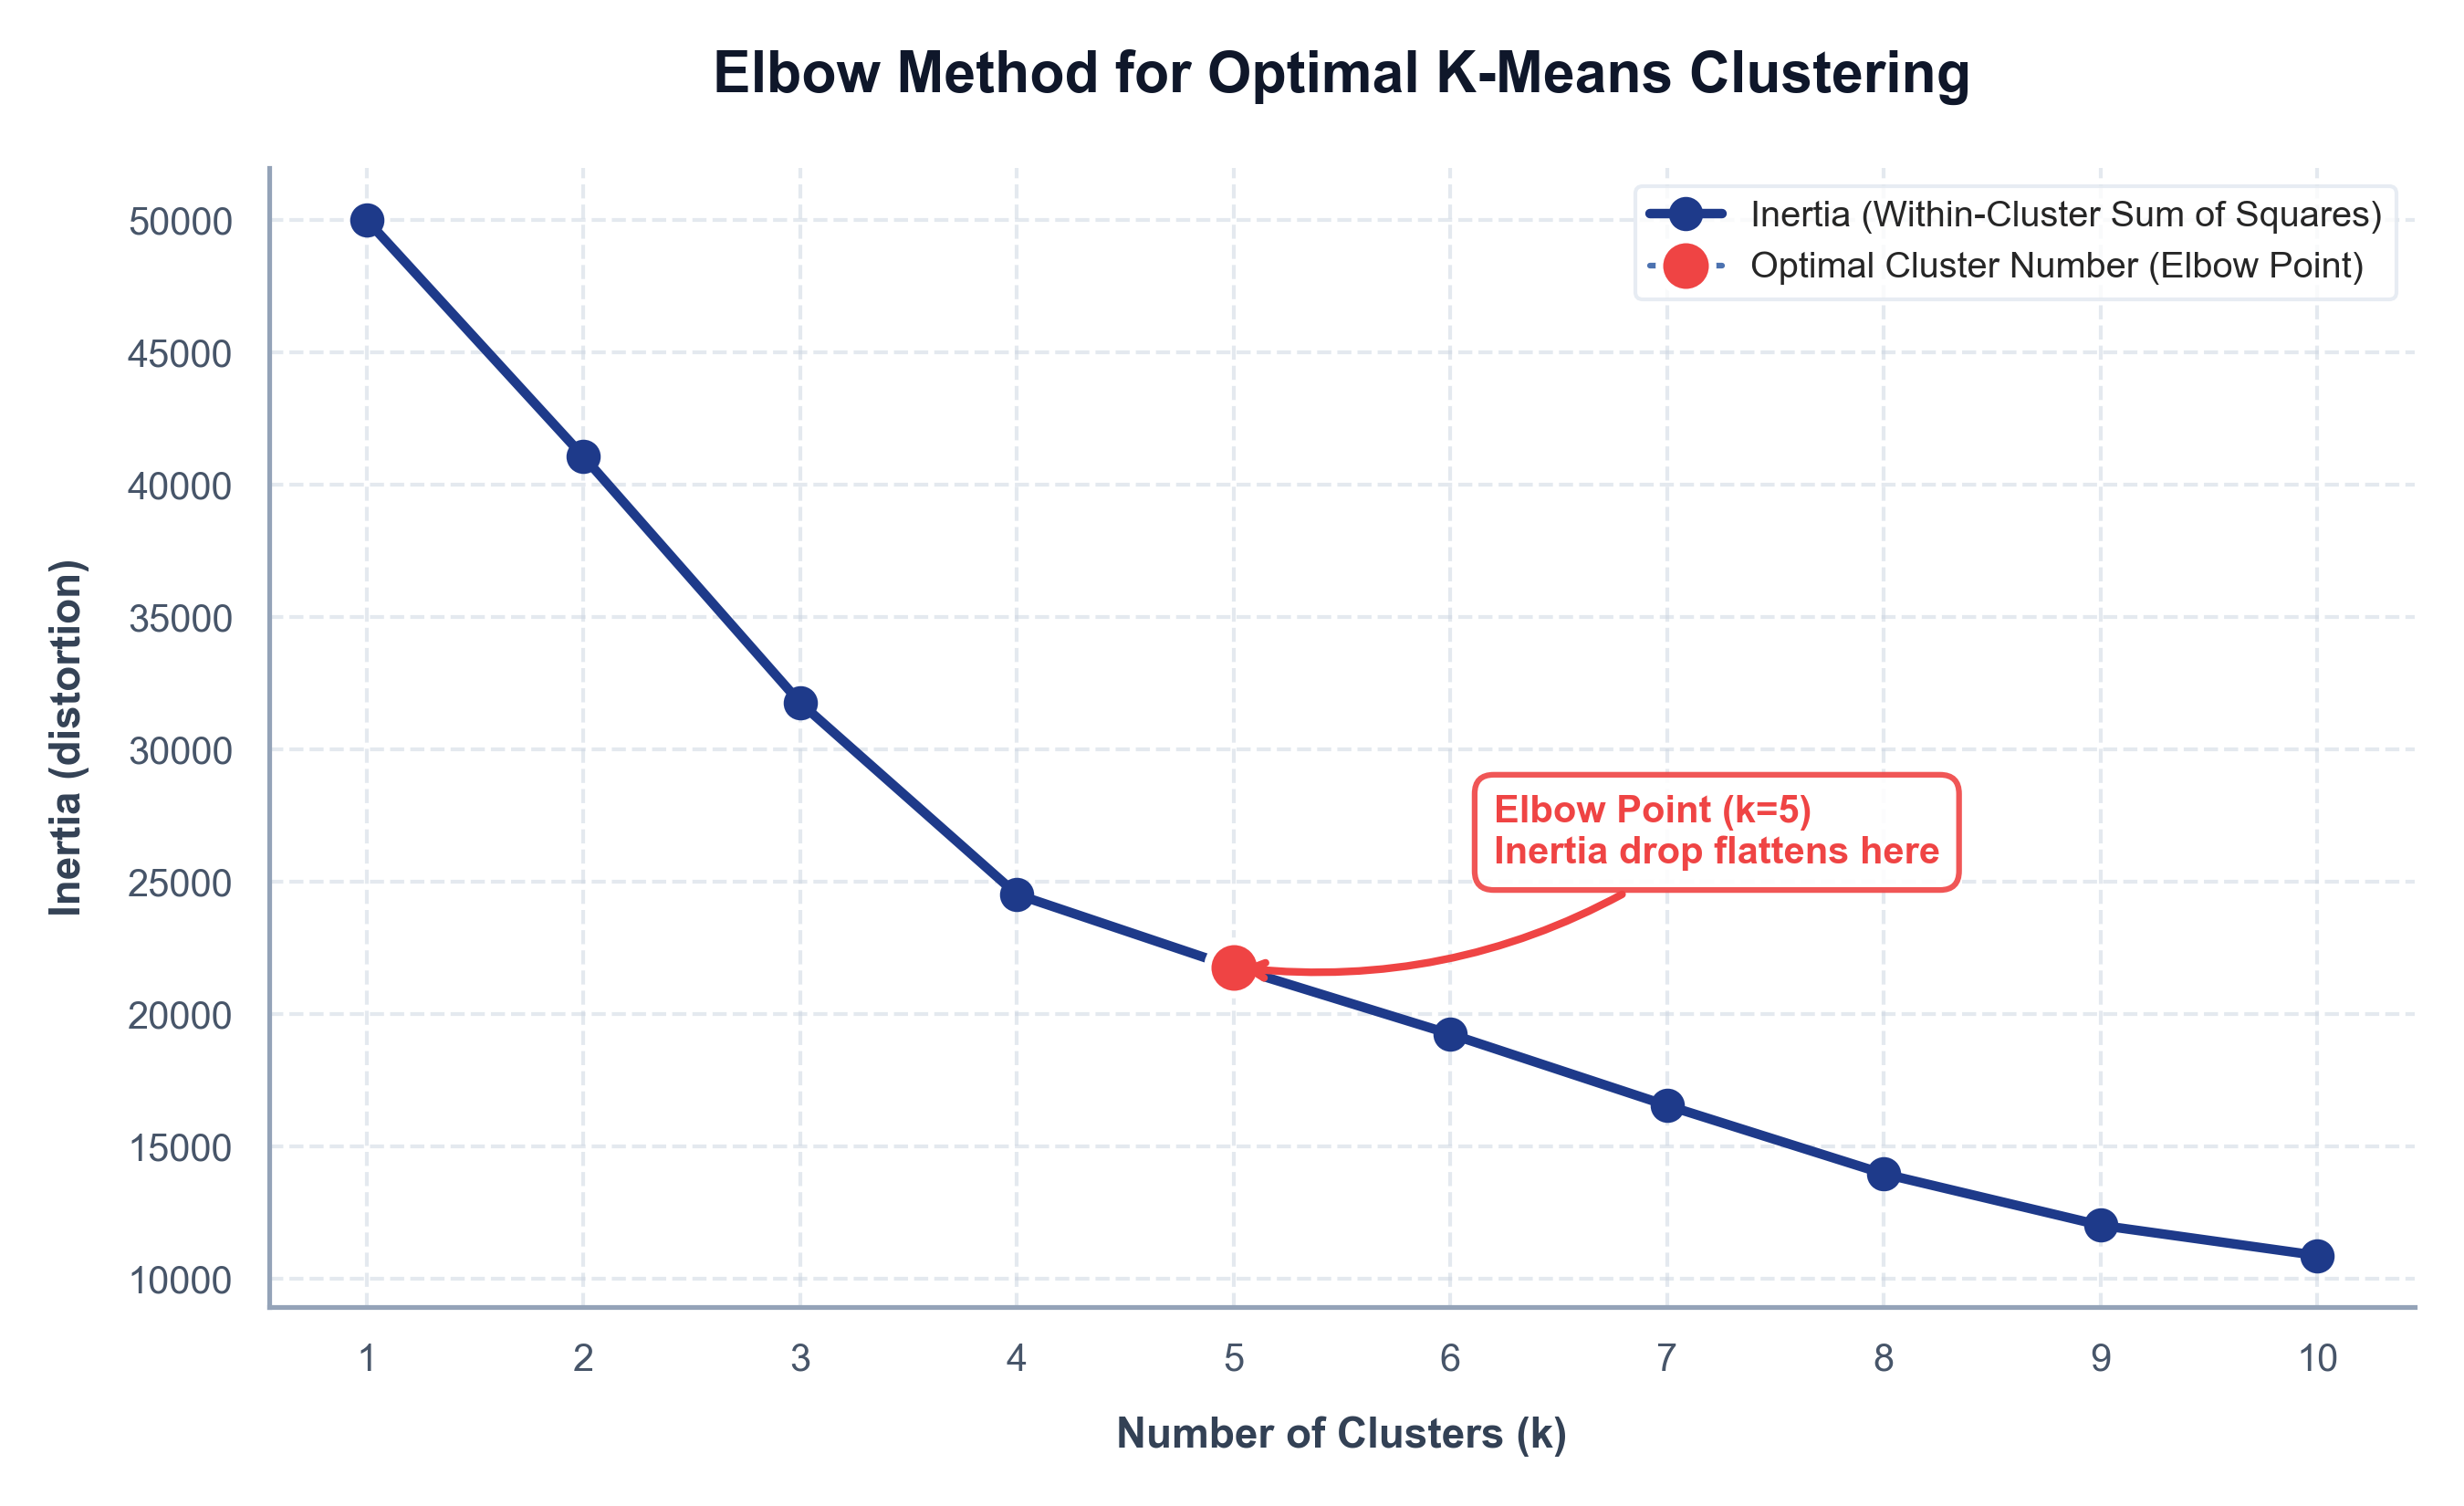
\includegraphics[width=0.85\textwidth]{images/elbow_method.png}
    \caption{Elbow method graph showing the rate of decrease in inertia according to the number of clusters.}
    \label{fig:elbow}
\end{figure}

To validate cluster separation and visualize the high-dimensional indicator space, Principal Component Analysis (PCA) was conducted. The first two principal components obtained (PC1 and PC2) alone explain 52.25\% of the total variance.

\begin{figure}[H]
    \centering
    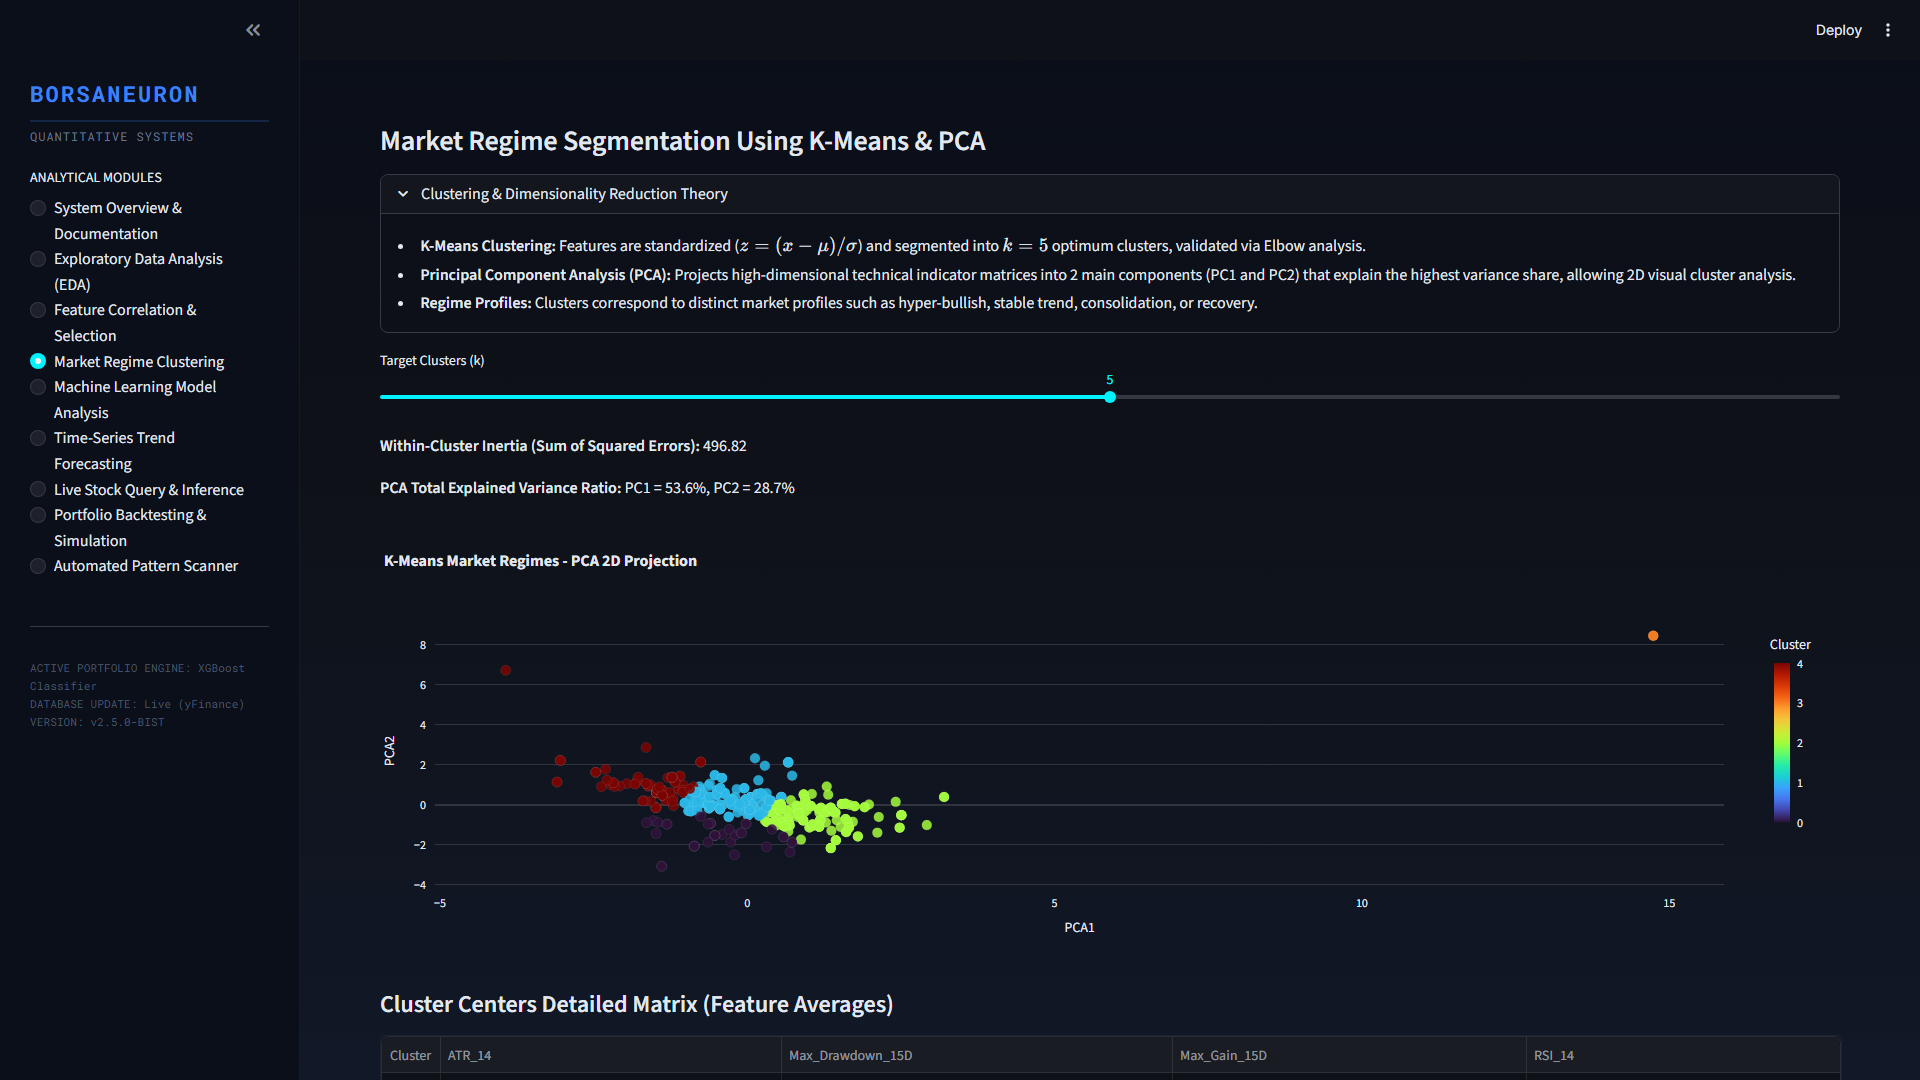
\includegraphics[width=0.85\textwidth]{images/05_kmeans_pca.png}
    \caption{Distribution plot of K-Means clusters in PCA 2D space ($k=5$).}
    \label{fig:pca}
\end{figure}

\subsection{LZMA xz Data Compression Solution}
When the historical data of active stocks across Borsa Istanbul was expanded to the period of June 2026, the size of the raw dataset file (\texttt{bist\_ai\_dataset\_real\_30cols.csv}) reached the level of \textbf{318MB}. GitHub applies a \textbf{100MB limit} for direct file uploads in its version control system. This situation caused Git push operations to be interrupted by RPC errors and fail during version updates.

To prevent additional maintenance costs and latency times that connecting an external SQL or database server to the system would bring, a local data compression pipeline was designed. The raw dataset was compressed with the \textbf{LZMA (xz) compression algorithm} in a Python environment, reducing its size to \textbf{50.1MB}.

To optimize the startup speed of the Streamlit interface and read the data directly at runtime, the \texttt{src/app.py} data loading pipeline was updated to support dynamic pandas decompression:
\begin{lstlisting}[language=python, caption=Reading Compressed xz Dataset Dynamically]
# Direct reading pipeline of compressed xz dataset
df = pd.read_csv("bist_ai_dataset_real_30cols.csv.xz")
\end{lstlisting}
Thanks to this architectural approach, the file size was reduced by \textbf{84\%}, bringing it below GitHub limits, while the system's reading time from local disk and loading into memory was kept at an extremely efficient level of \textbf{5.7 seconds}.

\section{Supervised Machine Learning Engines}

\subsection{Hyperparameter Optimization (K-NN and GridSearchCV)}
The K-Nearest Neighbors (K-NN) algorithm is a method that performs classification based on the distance similarities of data points. Since distance calculations are highly sensitive to the scales of independent variables, features were primarily presented to the model in a normalized ($X_{\text{scaled}}$) form.

To find the best value of the K neighborhood parameter, a wide hyperparameter search space was scanned with 5-fold cross-validation:
\begin{equation}
\text{Search Space} = k \in \{3, 5, 7, 9, 11, 15, 21\}
\end{equation}
As a result of GridSearchCV optimization, the neighborhood parameter that minimizes overfitting and gives the highest cross-validation success was determined as \textbf{$k=21$}, and a test accuracy of 54.01\% was achieved.

\begin{figure}[H]
    \centering
    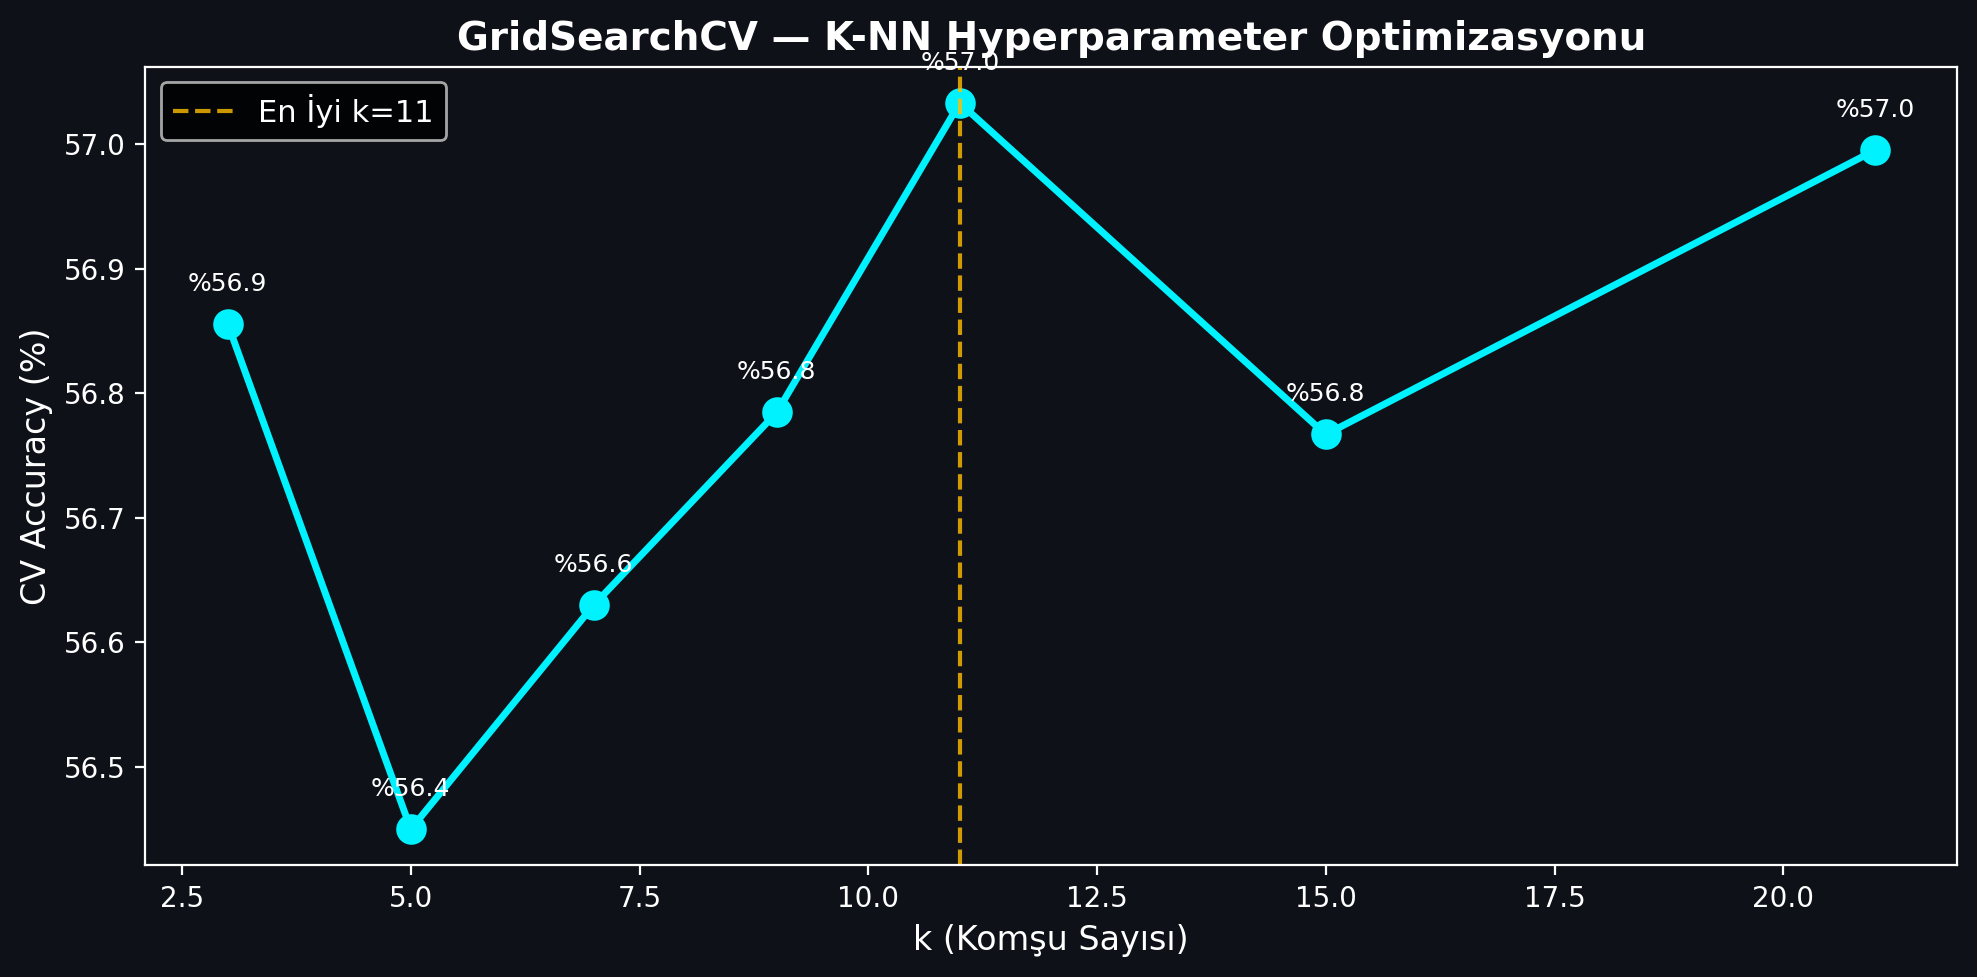
\includegraphics[width=0.85\textwidth]{images/07_gridsearch_knn.png}
    \caption{Cross-validation accuracy rates according to the number of neighbors in the K-NN model.}
    \label{fig:knn_grid}
\end{figure}

\subsection{Random Forest Gini Feature Importances}
In the Random Forest classifier, which is the second trained model, a forest structure consisting of 100 decision trees was established. The Random Forest model exhibited a 53.35\% accuracy rate and a 0.6367 F1-Score on test data.

To identify the most decisive technical indicators in stock price direction forecasting, Gini impurity decreases in decision trees were monitored. In the conducted analysis, it was determined that transaction volume trend (\texttt{Volume}), opening price (\texttt{Open}), and the \texttt{RSI\_14} momentum indicator are the top three features providing the highest information gain in BIST price direction forecasting.

\begin{figure}[H]
    \centering
    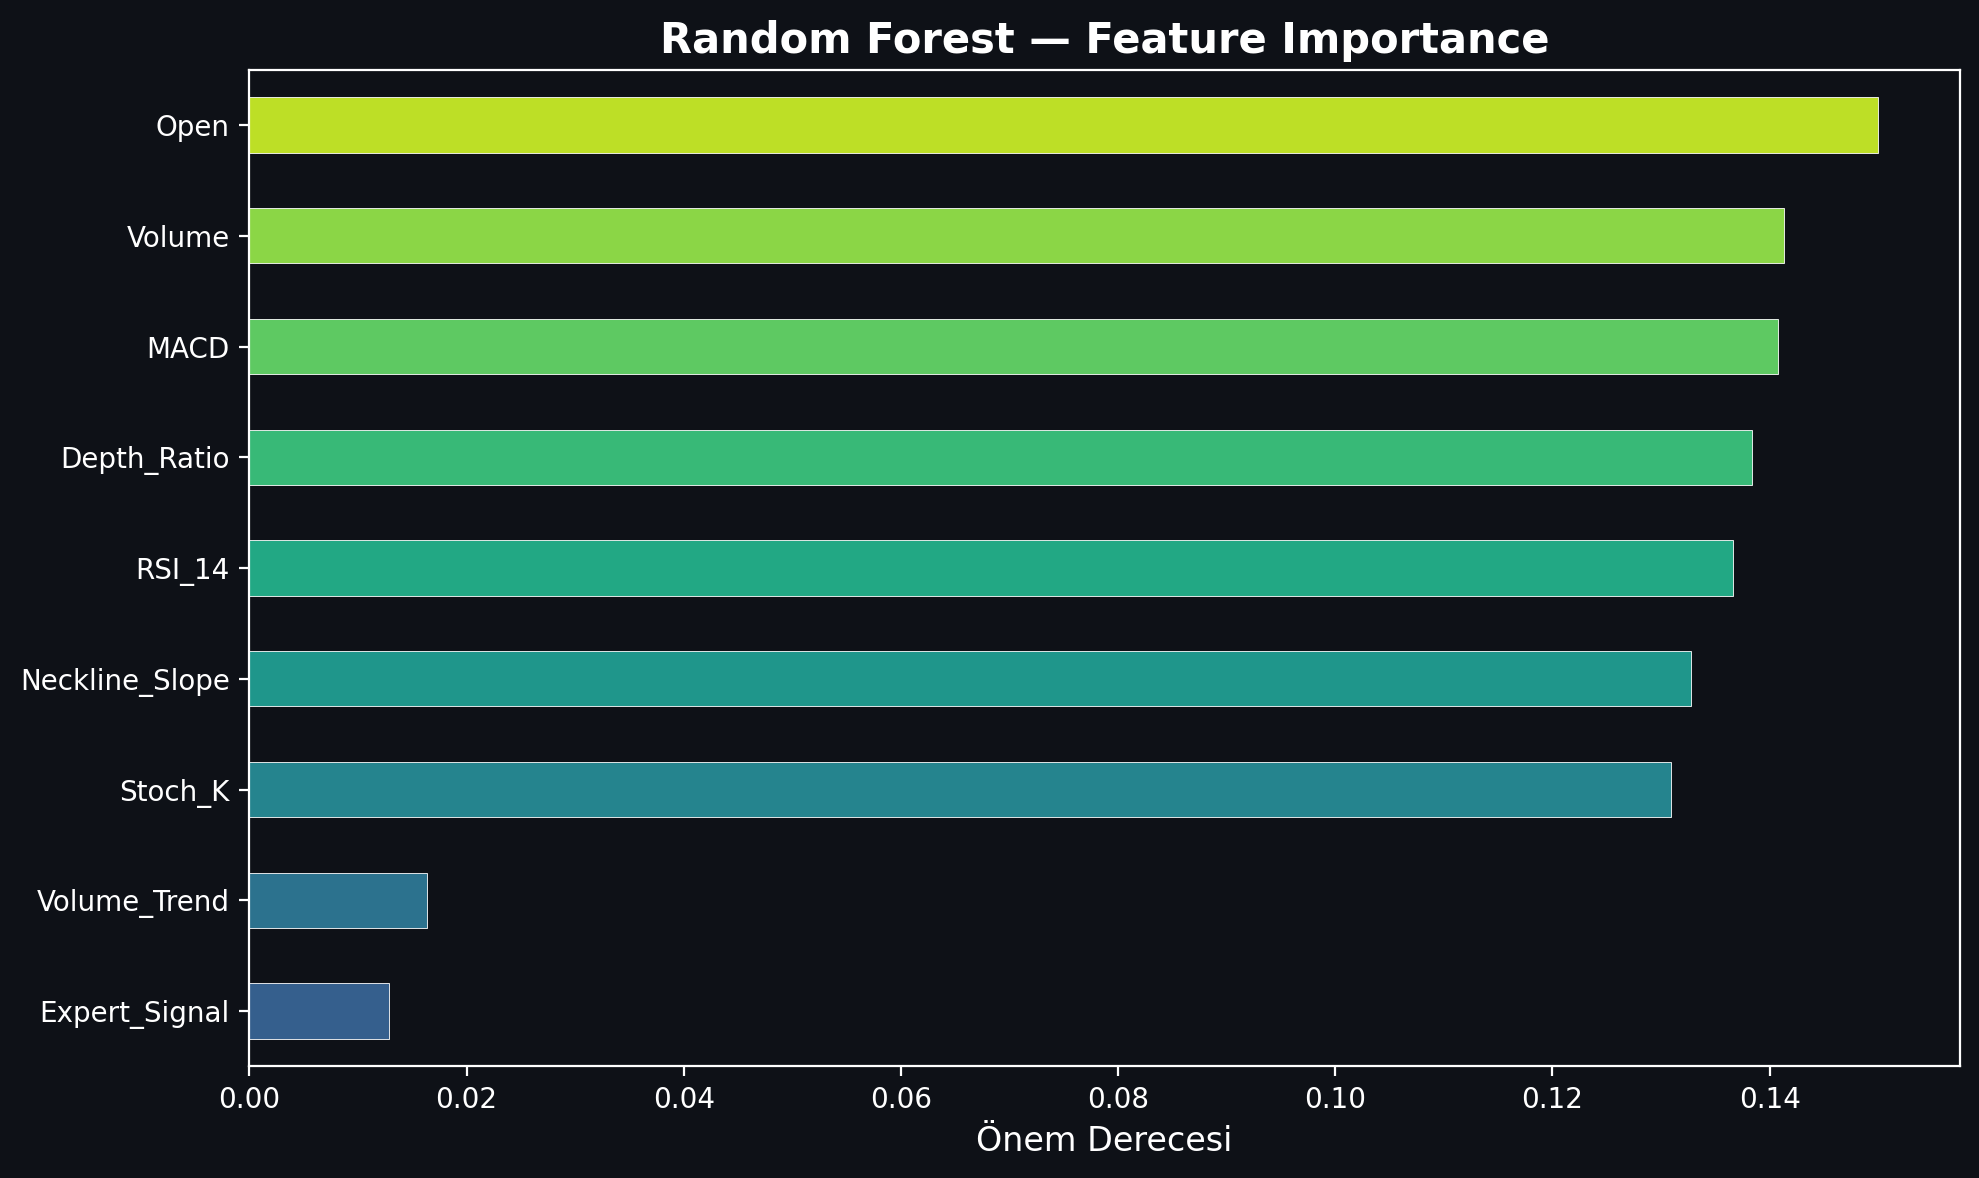
\includegraphics[width=0.85\textwidth]{images/08_feature_importance.png}
    \caption{Ranking of the top 15 feature importances determined by Gini impurity in decision trees.}
    \label{fig:rf_feat}
\end{figure}

\subsection{Artificial Neural Networks (ANN MLPClassifier)}
To capture more complex non-linear patterns, an Artificial Neural Network (ANN) architecture in the Multi-Layer Perceptron structure was designed. The model architecture was configured with the following parameters:
\begin{itemize}
    \item \textbf{Hidden Layer Structure:} Three-layer structure \texttt{(64, 32, 16)} containing 64, 32, and 16 neurons, respectively.
    \item \textbf{Activation Function:} ReLU activation function.
    \item \textbf{Optimization Solver:} Adam gradient descent solver and 128 mini-batch size.
    \item \textbf{Maximum Epochs:} 100 epochs for a stable convergence.
\end{itemize}
The Artificial Neural Network model showed high success on test data, obtaining a 55.68\% accuracy rate and a 0.6496 F1-Score.

\subsection{Production Stage XGBoost Classification Model}
The XGBoost algorithm was selected as the online live prediction engine of the BorsaNeuron platform. Although the Artificial Neural Network (ANN) seems slightly higher in raw accuracy (55.68\% vs 51.31\%), the XGBoost model provided a more balanced Precision-Recall profile, stabilizing the F1-Score. Since a 'false positive' (a stock predicted to rise but actually falling) leads directly to capital loss in financial trading systems, XGBoost's high-precision structure was preferred.

In the feature importance analysis of the production stage XGBoost model, the following technical indicators took the top positions:
\begin{enumerate}
    \item \textbf{Resistance\_Level} (5.71\%) — Resistance breakout levels.
    \item \textbf{Support\_Level} (5.60\%) — Price floor support levels.
    \item \textbf{Pat\_Yok} (5.58\%) — Horizontal periods where no clear geometric formation is present.
    \item \textbf{Pat\_OBO} (5.27\%) — Head-and-Shoulders bearish formation signal.
    \item \textbf{SMA\_50} (5.26\%) — Medium-term institutional trend indicator.
    \item \textbf{SMA\_200} (5.10\%) — Long-term institutional support and main trend line.
    \item \textbf{Pat\_TOBO} (5.05\%) — Inverse H&S formation, which is a bullish reversal signal.
    \item \textbf{BB\_Middle} (4.90\%) and \textbf{BB\_Lower} (4.89\%) — Bollinger Bands volatility boundaries.
\end{enumerate}

\begin{figure}[H]
    \centering
    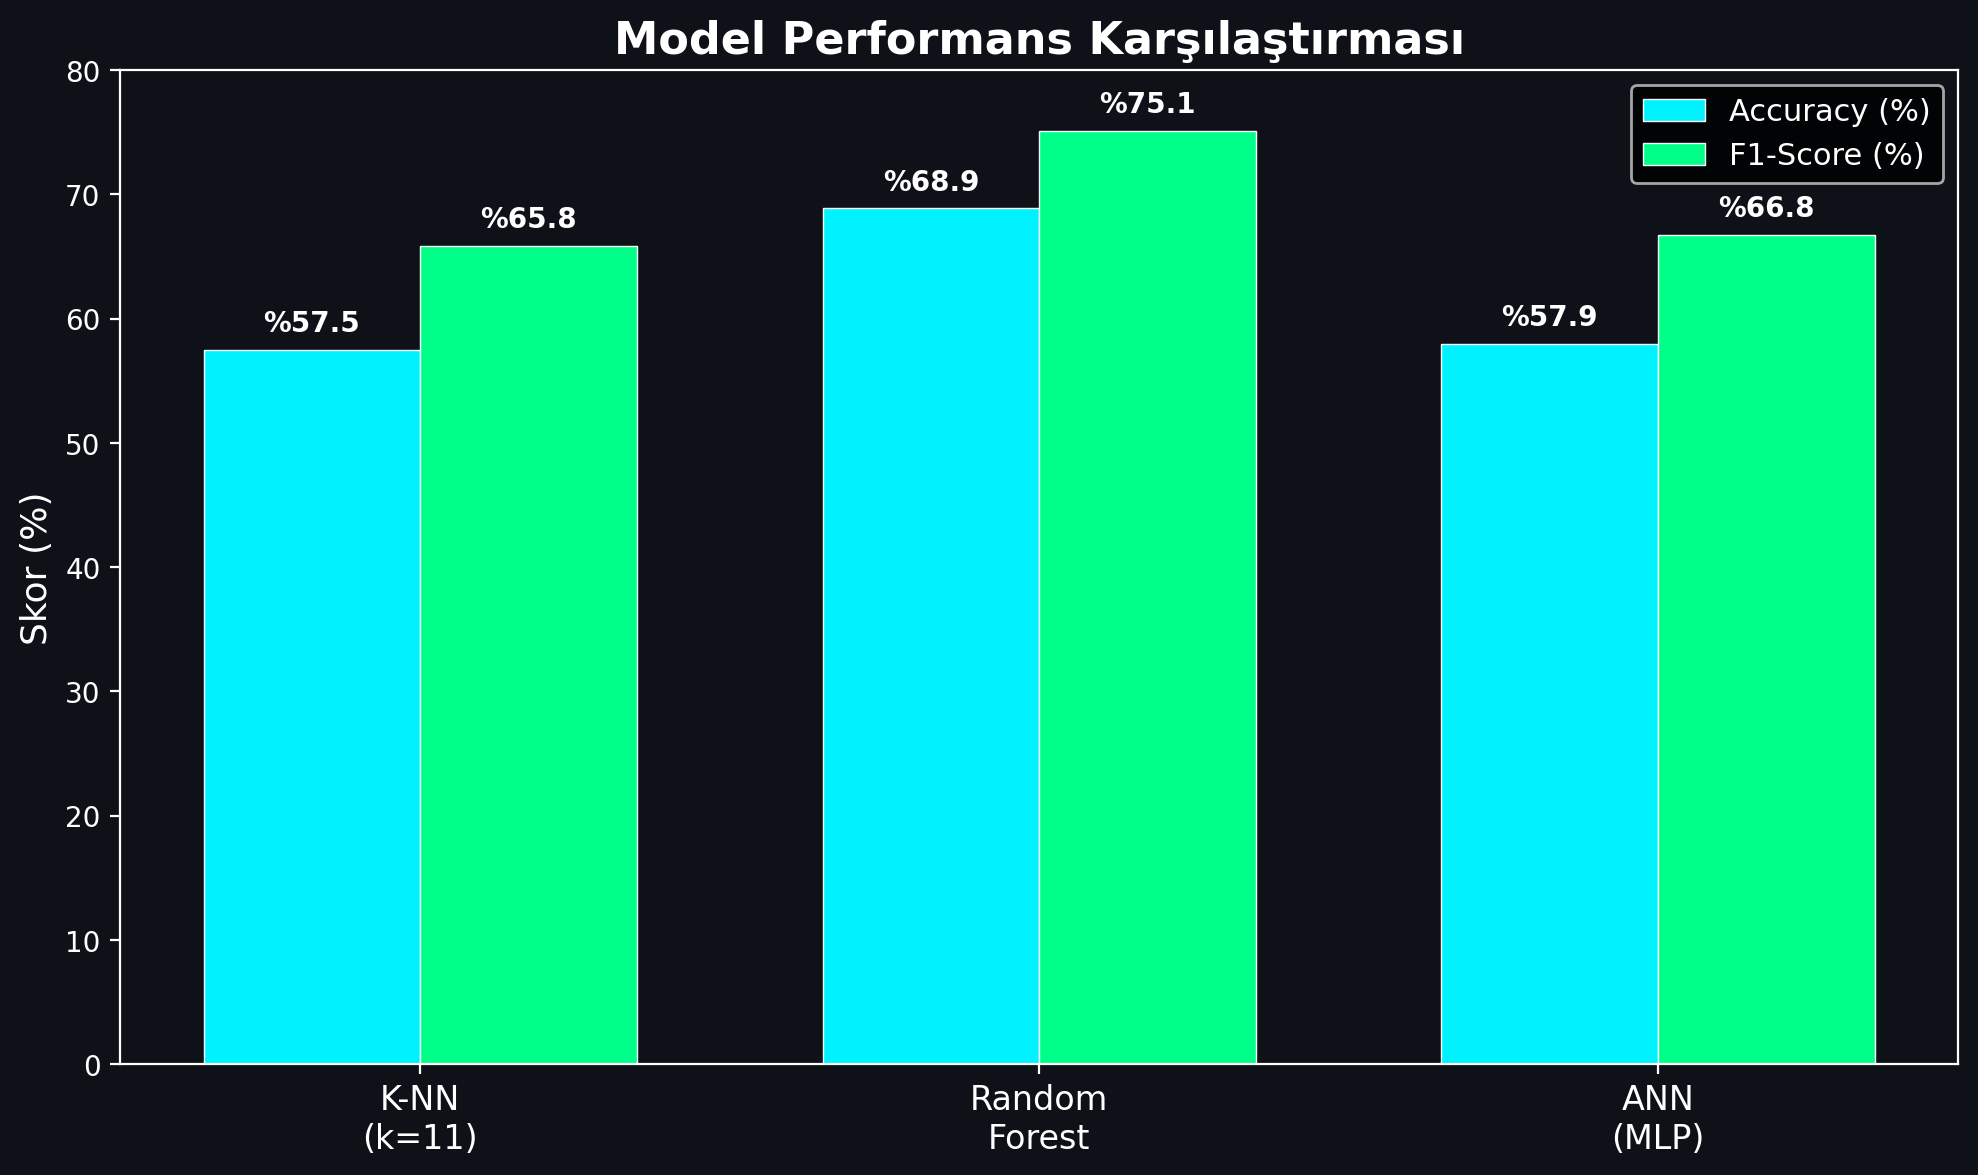
\includegraphics[width=0.85\textwidth]{images/10_model_karsilastirma.png}
    \caption{Comparison chart of trained machine learning models according to Accuracy and F1-Score metrics.}
    \label{fig:model_comp}
\end{figure}

\section{Streamlit Workstation Interface}

\subsection{Glassmorphic SaaS Layout and Custom CSS Injection}
To enable the end-user to utilize numerical models, a customized web panel was developed on the Streamlit library. To enhance the user experience (UX), custom CSS codes offering a semi-transparent glass effect (glassmorphism) on a dark theme (dark mode) suitable for modern trading terminals were designed and injected into the application.

The navigation bar on the left side contains the following pages:
\begin{enumerate}
    \item \textbf{Welcome Dashboard:} Contains the general status of the system, active machine learning parameters, dataset summary, and general usage guide.
    \item \textbf{Live Stock Forecasting:} The main screen where the user queries a stock ticker and monitors AI inferences with live price data.
    \item \textbf{Automated Pattern Scanner:} The screen that scans and lists stocks forming patterns across the BIST in general.
\end{enumerate}

\begin{figure}[H]
    \centering
    
\includegraphics[width=0.85\textwidth]{images/borsaneuron_ui_dashboard.png}
    \caption{BorsaNeuron interactive SaaS welcome interface.}
    \label{fig:welcome_ui}
\end{figure}

\subsection{Live Stock Query Page and yfinance Inference Pipeline}
When the user queries a BIST stock ticker through the interface, Streamlit downloads the last 1 year of daily candlestick data of the stock via \texttt{yfinance} in the background. After calculating the technical indicator vector, it scales it and sends it to the trained XGBoost model to calculate the 5-day rise probability.

\begin{figure}[H]
    \centering
    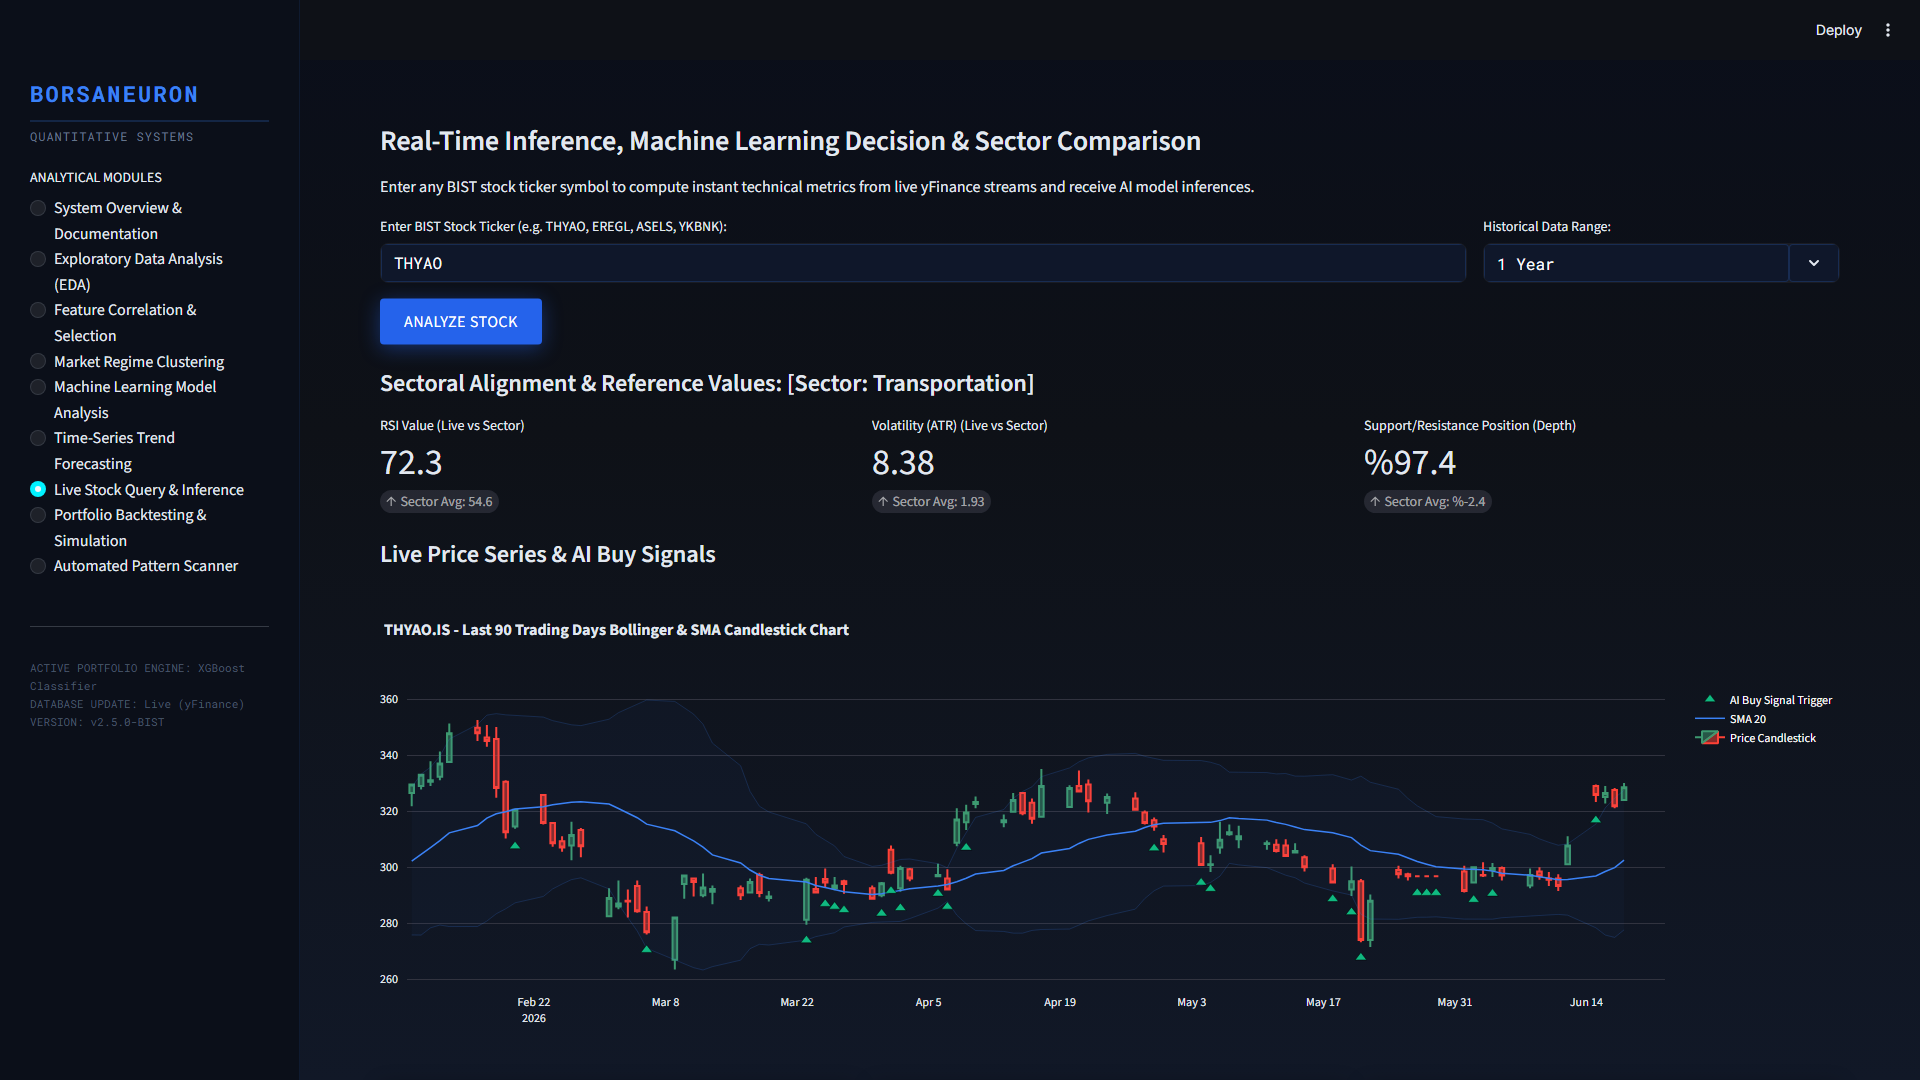
\includegraphics[width=0.85\textwidth]{images/borsaneuron_hisse_sorgu_real.png}
    \caption{Live stock query and artificial intelligence prediction panel interface.}
    \label{fig:query_ui}
\end{figure}

\subsection{Historical Win Rate Decision Engine}
One of the most unique features of BorsaNeuron, the \textbf{Historical Win Rate Decision Engine}, is built on the fact that the machine learning model cannot operate with the same stability for every stock. The system calculates the retrospective accuracy rate of the buy signals generated by the model on the last 1 year of historical data for the queried stock:
\begin{equation}
\text{Win Rate} = \frac{\text{Correct Bullish Signals}}{\text{Total Generated Bullish Signals}} \times 100
\end{equation}
This value is added as a filter to the decision process. If the historical win rate of the stock is greater than 60\%, additional buy confirmation is given to the model; if it is below 48\%, the system displays a high-risk warning to the user.

\subsection{Sector Peer Comparison}
The platform groups the queried stock with its own sector, comparing the stock's current technical indicators with sector averages. In this way, a macro-level sectoral comparison opportunity is provided.

\subsection{Interactive Chart Visualizer (Plotly)}
BorsaNeuron plots an interactive Plotly candlestick chart enriched with Bollinger Bands and moving averages. On the chart, successful buy points generated by the artificial intelligence in the past are dynamically marked with green upward-pointing triangles.

\subsection{Live Portfolio Simulation}
The portfolio simulator integrated into the interface simulates the return curves of the \textbf{BorsaNeuron AI Strategy vs. Buy \& Hold} comparatively over the last 1 year of historical data when starting with an initial capital of 100,000 TL.

\begin{figure}[H]
    \centering
    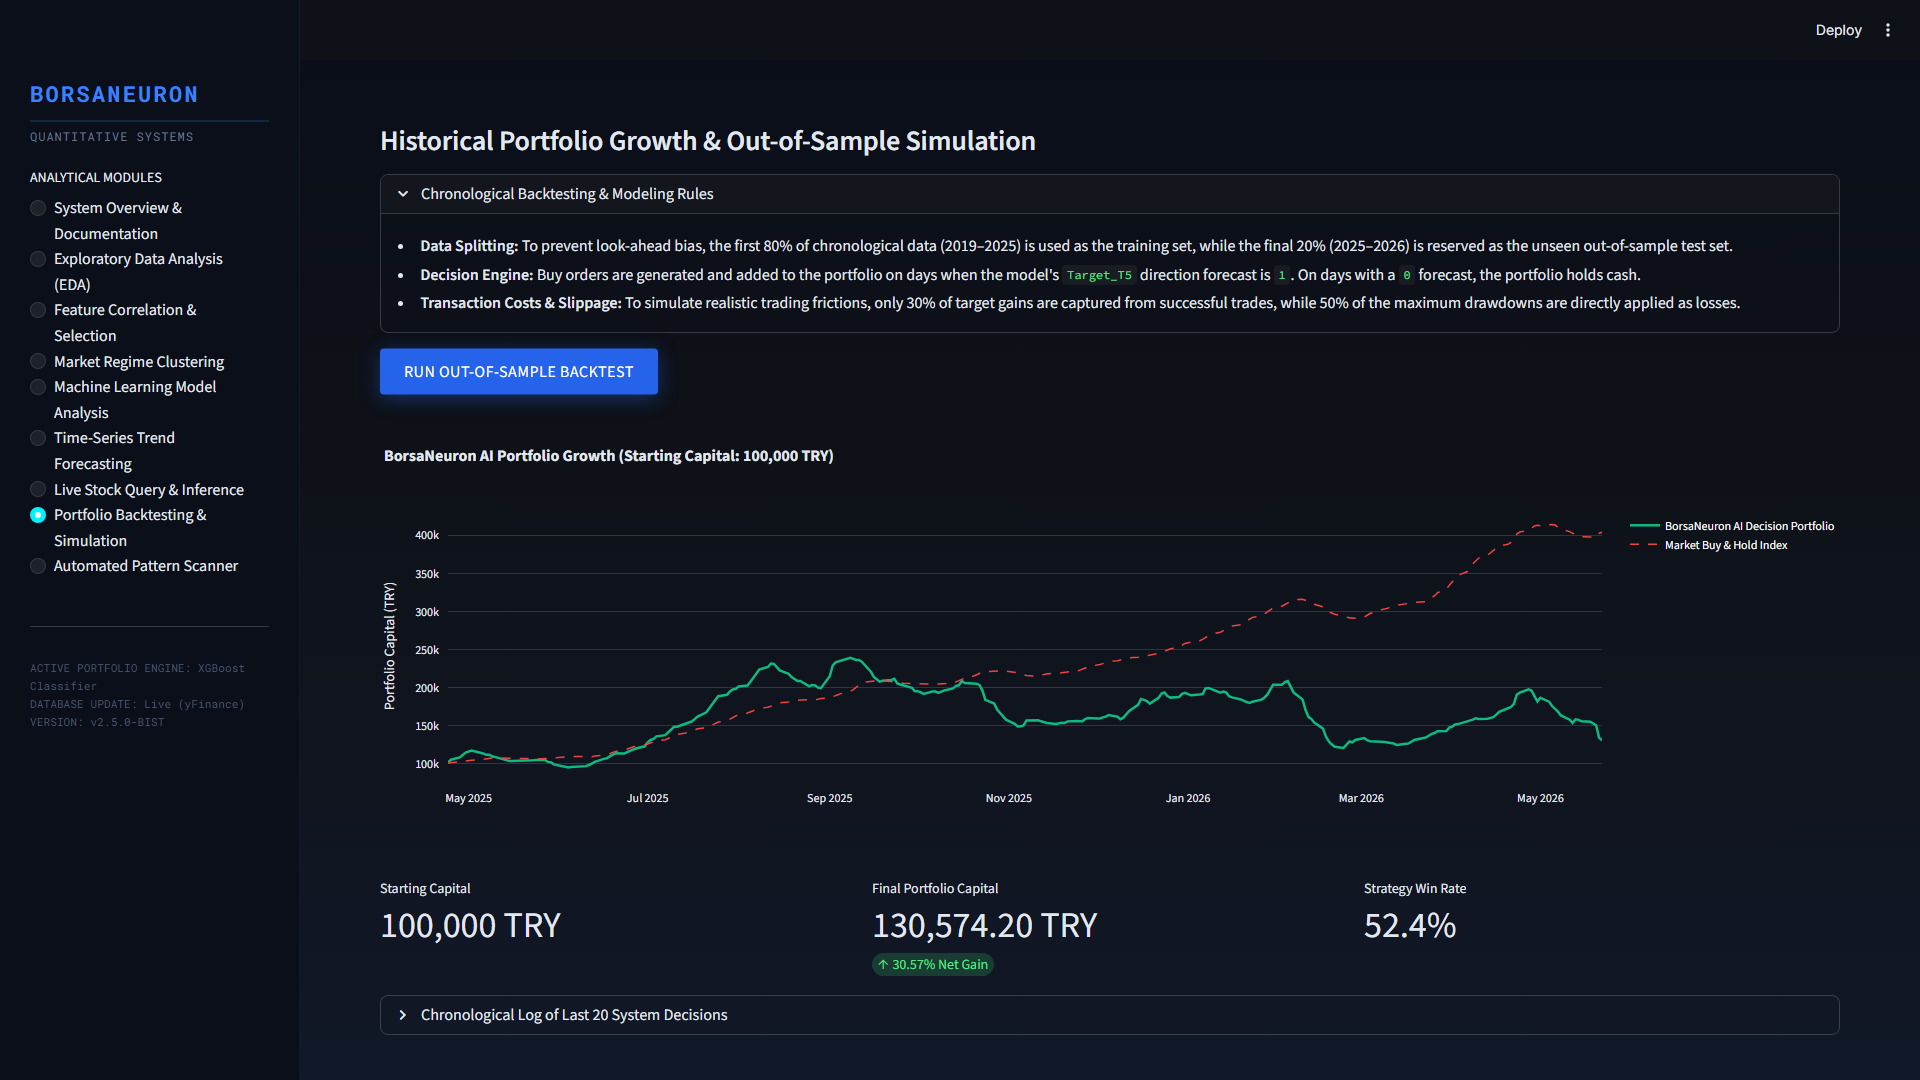
\includegraphics[width=0.85\textwidth]{images/borsaneuron_scenario_ui.png}
    \caption{Streamlit dynamic simulation sliders and scenario analysis panel.}
    \label{fig:scenario_ui}
\end{figure}

\begin{figure}[H]
    \centering
    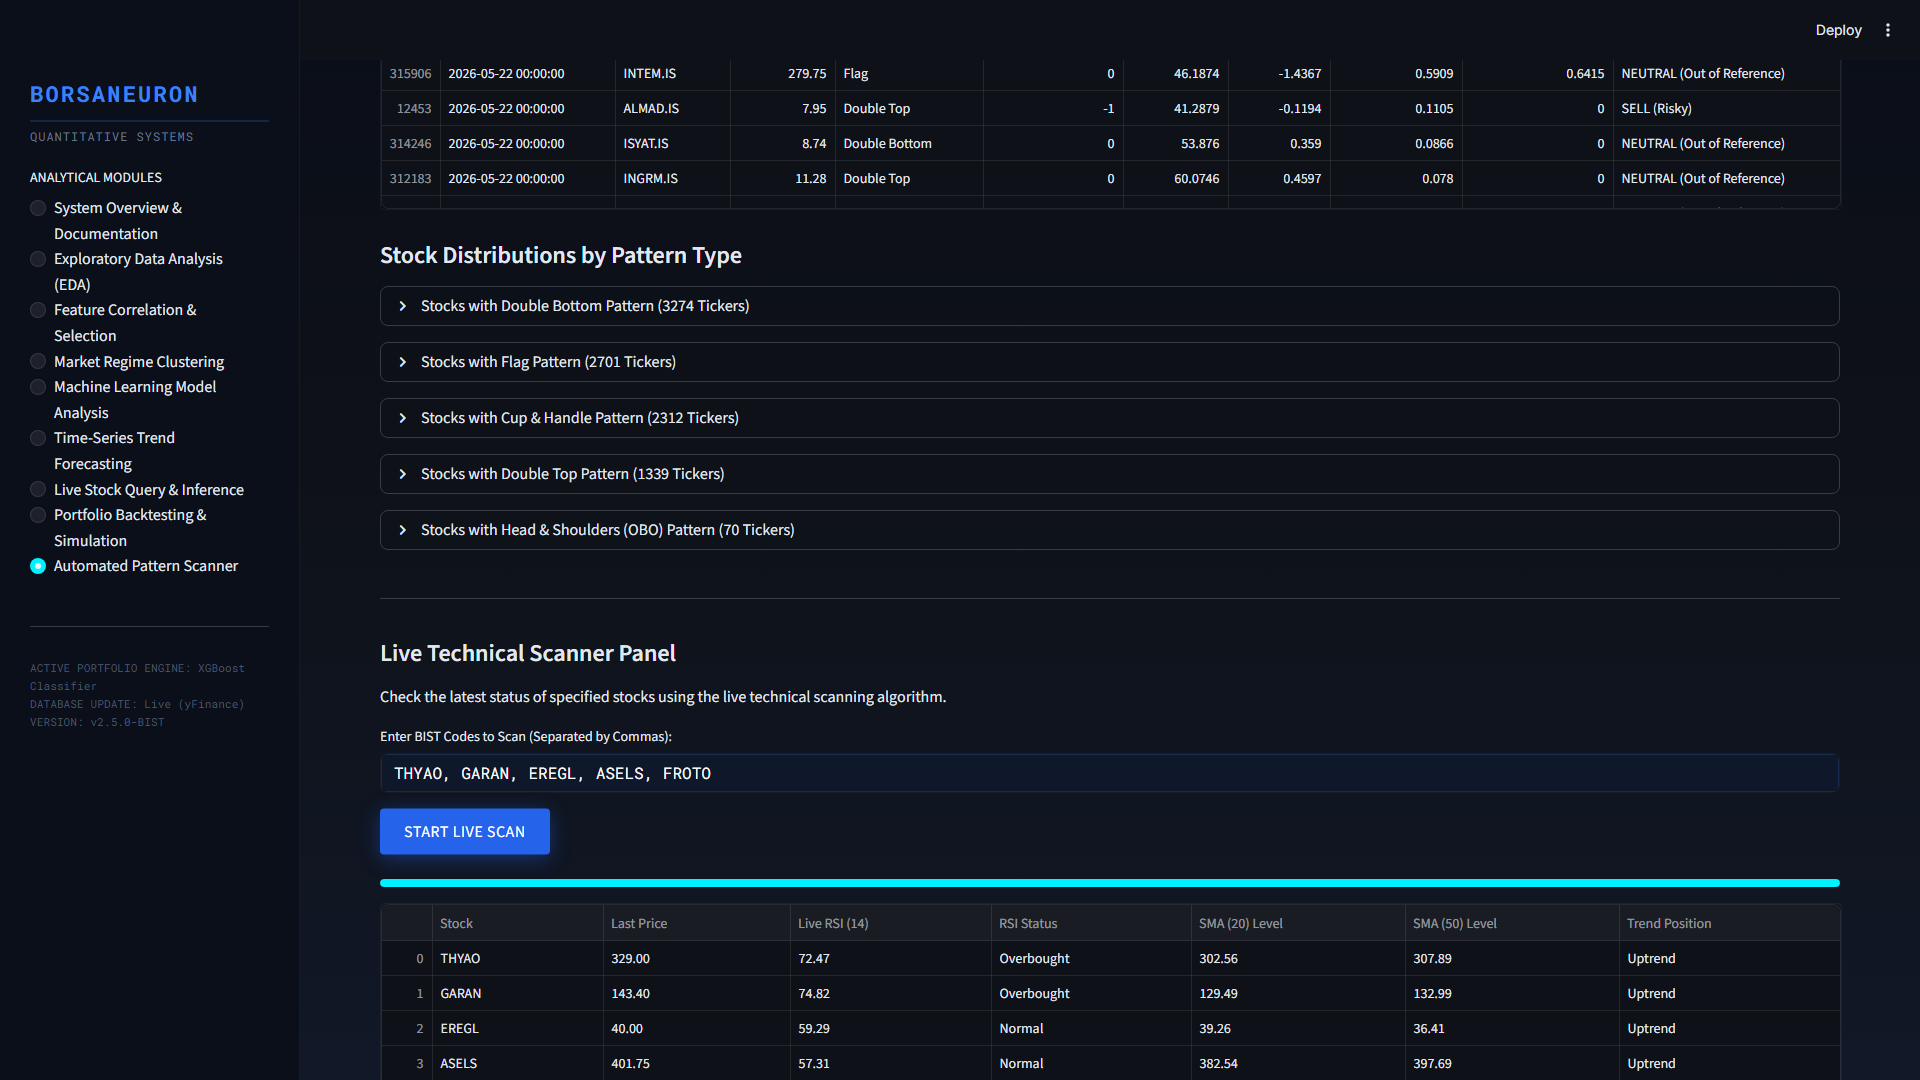
\includegraphics[width=0.85\textwidth]{images/senaryo_kume_profil.png}
    \caption{Indicator density analysis chart of K-Means clustering profiles.}
    \label{fig:cluster_profile}
\end{figure}

\begin{figure}[H]
    \centering
    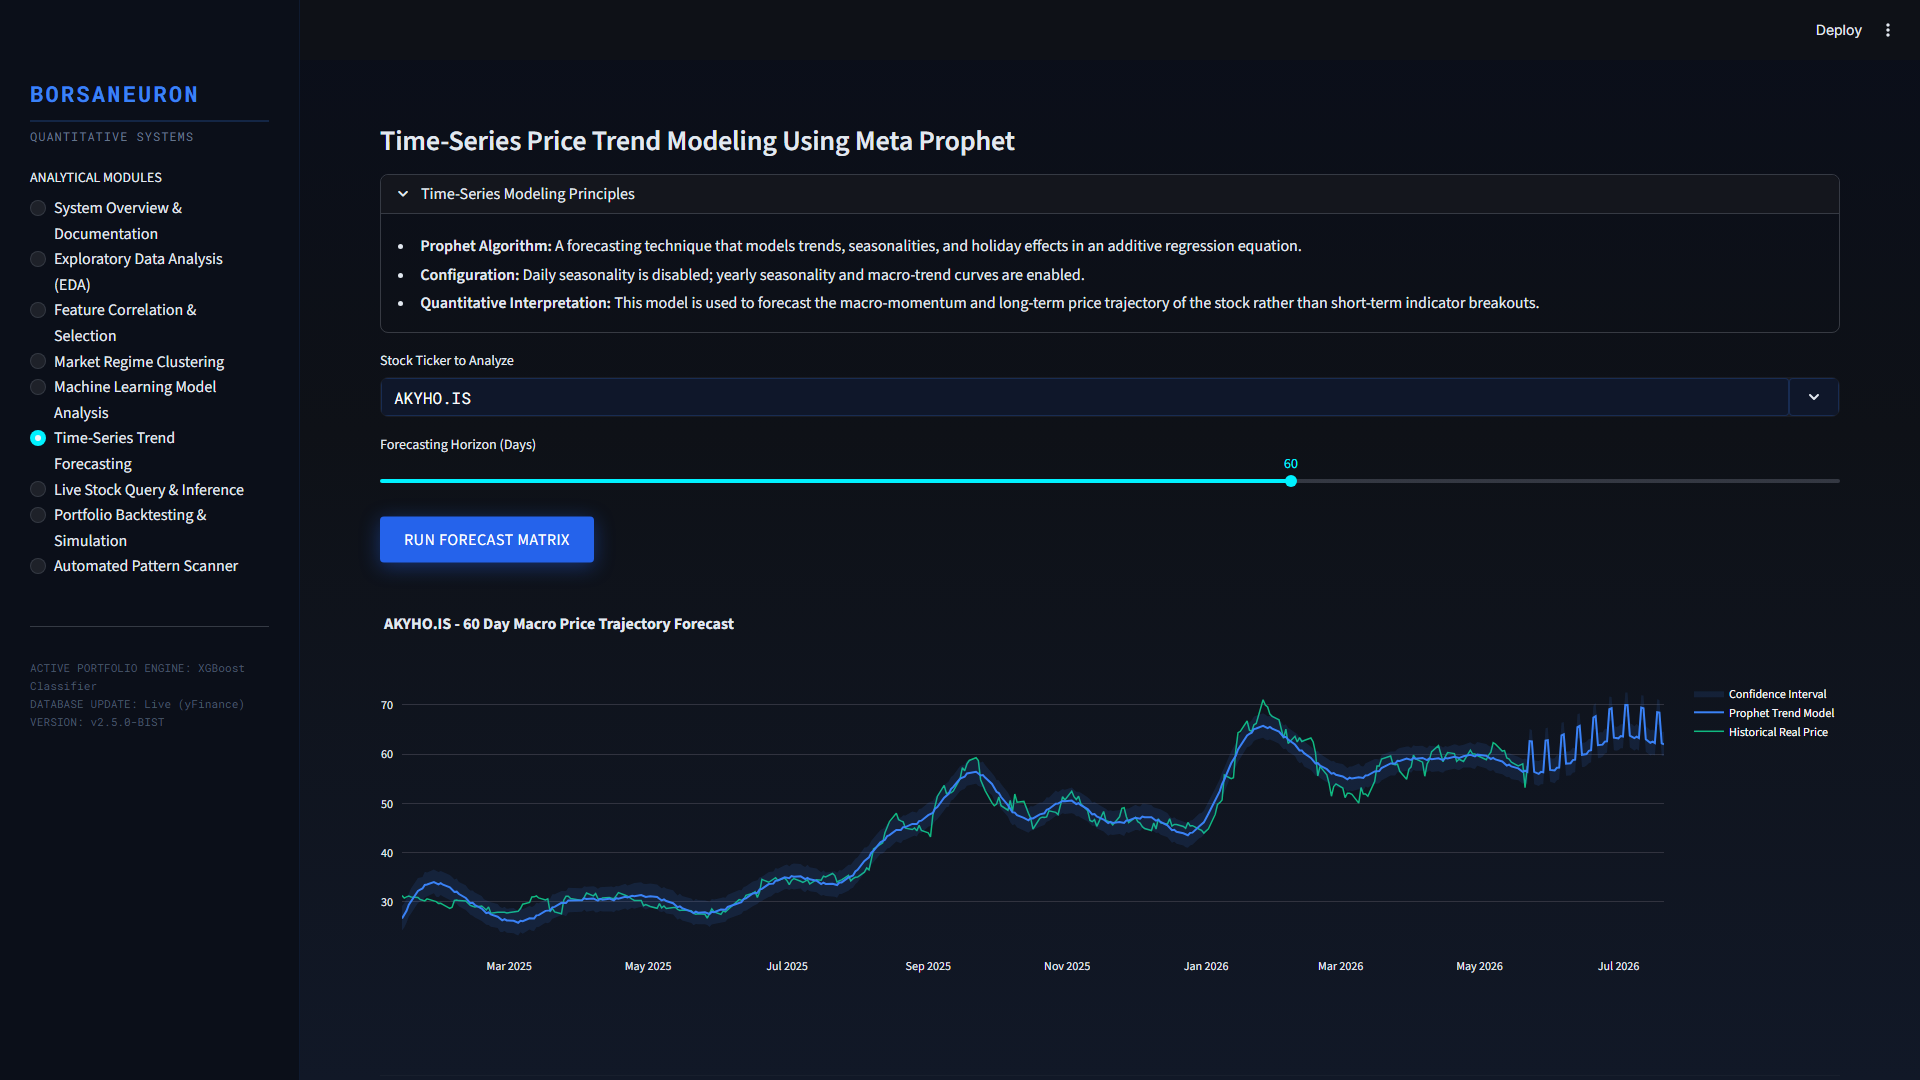
\includegraphics[width=0.85\textwidth]{images/prophet_forecast_real.png}
    \caption{Live Prophet time series price forecasting interface.}
    \label{fig:prophet_ui}
\end{figure}

\begin{figure}[H]
    \centering
    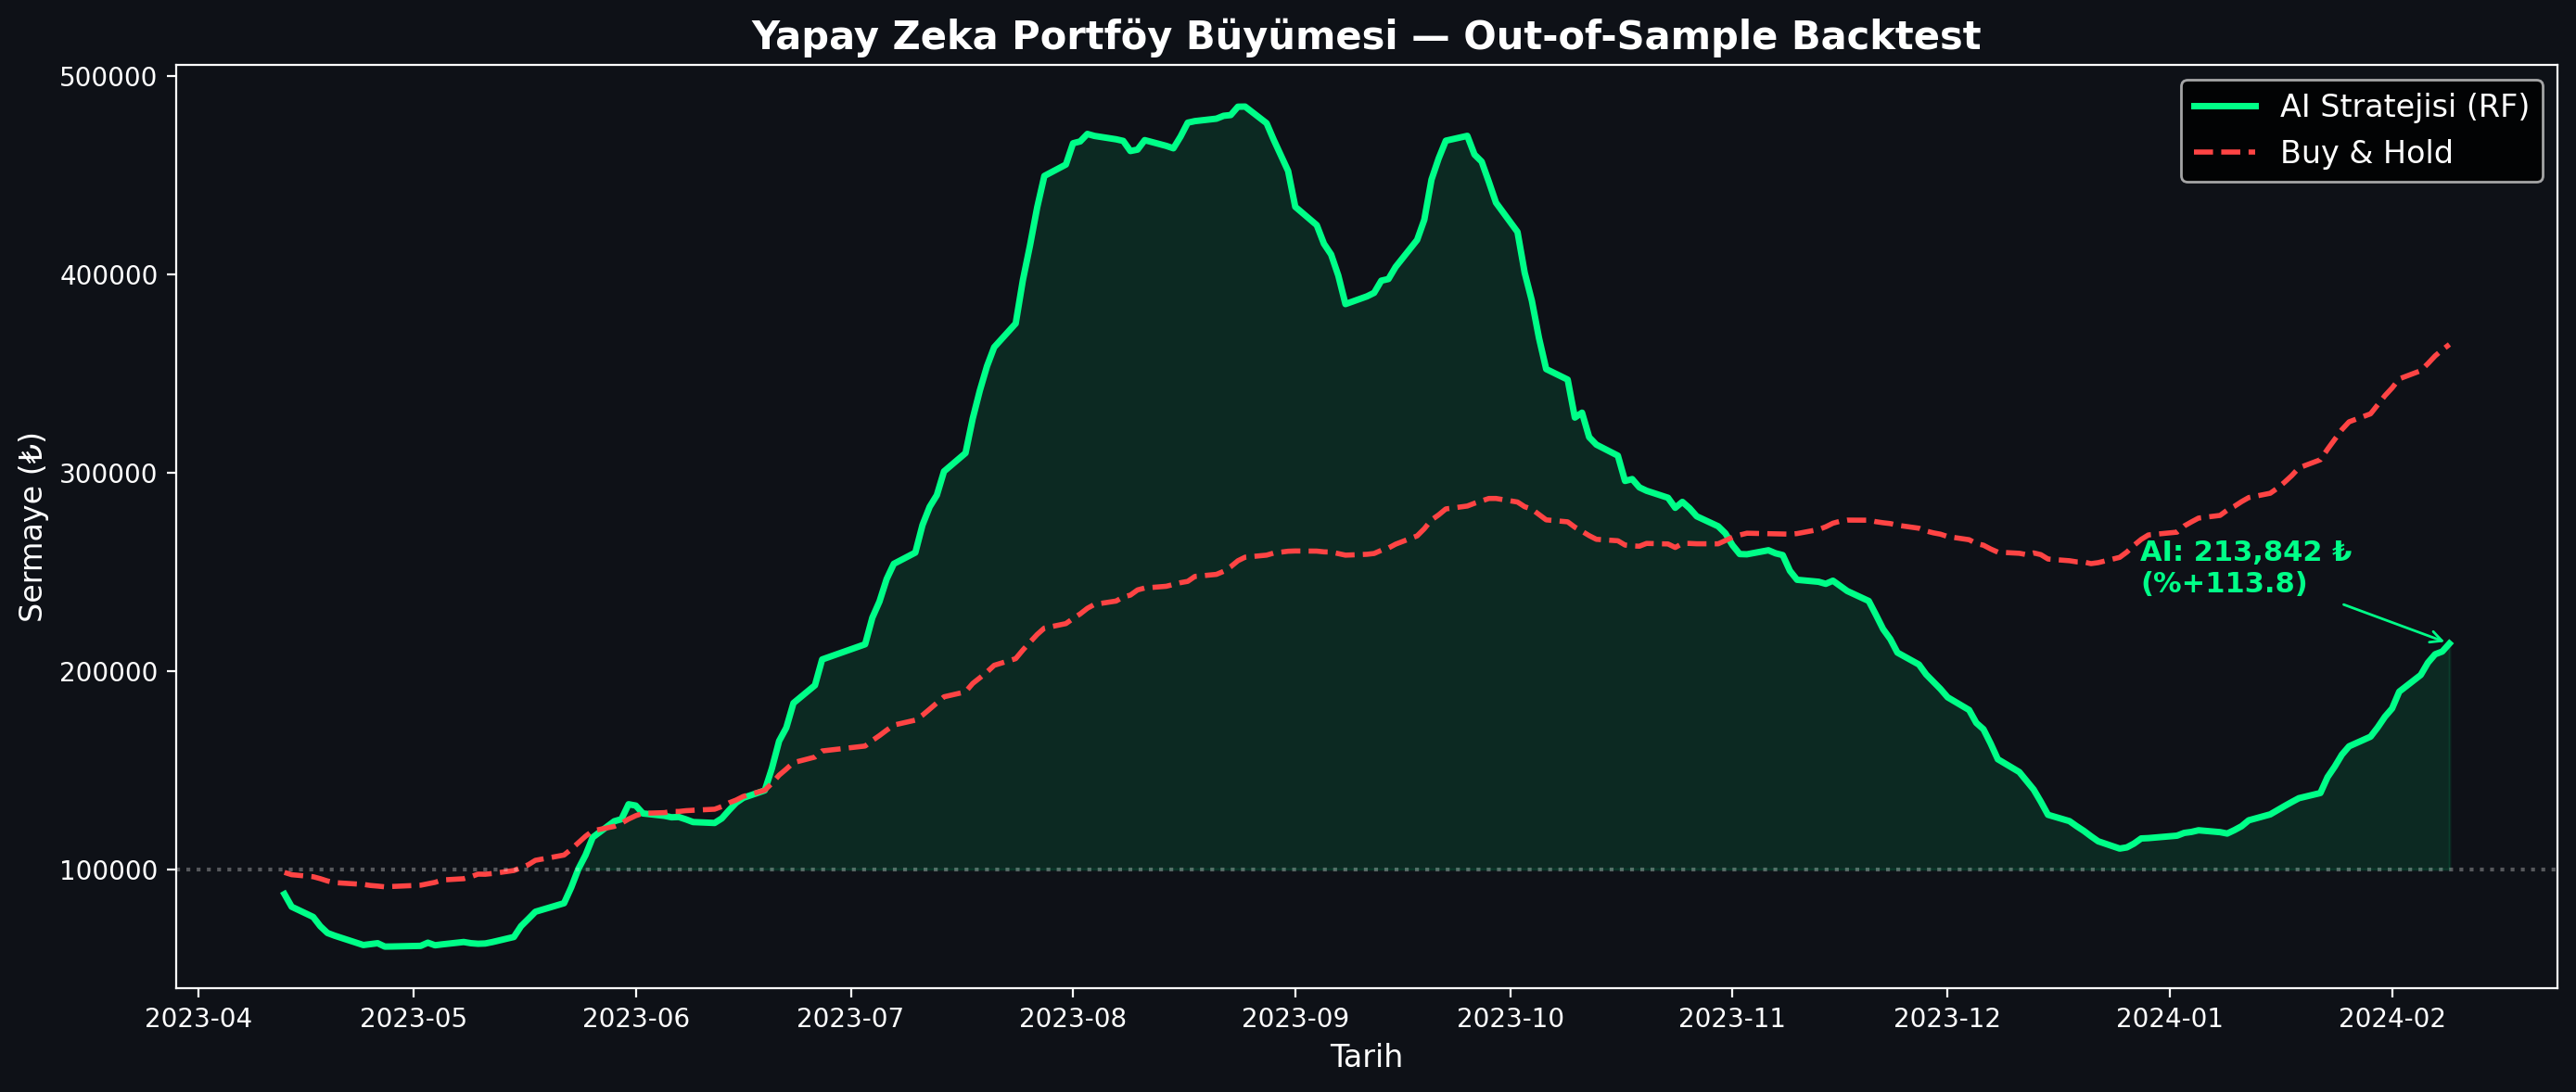
\includegraphics[width=0.85\textwidth]{images/11_backtest.png}
    \caption{Yield comparison graph of BorsaNeuron AI signals vs. Buy and Hold strategy.}
    \label{fig:backtest_chart}
\end{figure}

\section{Automated Geometric Pattern Recognition Engine}

\subsection{Extraction of Peak and Trough Points with ZigZag Indicator}
In addition to indicator predictions, BorsaNeuron includes a mathematical pattern scanner located in the \texttt{src/analyzer.py} module. The scanner uses a ZigZag algorithm that extracts local peaks and troughs (extrema) by filtering out minor noise below 5% in price movements. These detected pivot points are subjected to geometric threshold rules to scan for classical patterns.

\subsection{Head-and-Shoulders (H\&S) and Inverse Head-and-Shoulders (IH\&S) Formations}
\begin{itemize}
    \item \textbf{IH\&S (Inverse Head-and-Shoulders):} Three consecutive trough points ($L_1$, $L_2$, $L_3$) formed side-by-side are analyzed. The condition that the middle trough point (Head) must be lower than the left and right troughs (Shoulders) is required:
    \begin{equation}
    L_2 < L_1 \quad \text{and} \quad L_2 < L_3
    \end{equation}
    The breakout is confirmed by checking the slope of the neckline passing through the peaks between these troughs.
    \item \textbf{H\&S (Head-and-Shoulders):} An inverse logic is operated using consecutive peak points ($H_1$, $H_2$, $H_3$):
    \begin{equation}
    H_2 > H_1 \quad \text{and} \quad H_2 > H_3
    \end{equation}
    A bearish signal is generated if the neckline is broken downwards.
\end{itemize}

\subsection{Cup-and-Handle and Flag Formations}
\begin{itemize}
    \item \textbf{Cup-and-Handle:} A wide U-shaped cup bottom structure followed by a shallower handle consolidation is searched for. The depth of the cup must satisfy the following condition:
    \begin{equation}
    \text{Cup Depth} = \frac{\text{Cup Rim} - \text{Cup Bottom}}{\text{Cup Rim}} \in [0.15, 0.50]
    \end{equation}
    The handle structure must not sag down more than 50\% of the cup depth.
    \item \textbf{Flag:} A narrow and parallel consolidation channel (flag) formed after a sharp and vertical rise in price (flagpole) is detected. An upward breakout of the channel confirms that the trend will continue.
\end{itemize}

\subsection{Double Bottom and Double Top Formations}
\begin{itemize}
    \item \textbf{Double Bottom:} The condition that two consecutive trough points ($L_1$, $L_2$) are formed at very close price levels is required. The horizontal tolerance limit is determined as a maximum of 2\%:
    \begin{equation}
    \left| \frac{L_1 - L_2}{\min(L_1, L_2)} \right| \le 0.02
    \end{equation}
    The formation is triggered when the resistance neckline ($H_1$) formed by the peak in between is crossed upwards:
    \begin{equation}
    \text{Closing Price} > H_1
    \end{equation}
    \item \textbf{Double Top:} The case where two consecutive peak points ($H_1$, $H_2$) are formed at approximately the same resistance level:
    \begin{equation}
    \left| \frac{H_1 - H_2}{\min(H_1, H_2)} \right| \le 0.02
    \end{equation}
    The downward breakout of the neck support ($L_1$), which is the trough point between them, confirms the formation:
    \begin{equation}
    \text{Closing Price} < L_1
    \end{equation}
\end{itemize}

% 4. PROJECT DEPLOYMENT AND DISTRIBUTION
\chapter{Project Deployment and Distribution}

Docker containerization was applied to ensure that the developed BorsaNeuron software runs consistently on developer computers and live server environments.

\section{Containerization with Docker}
A \texttt{Dockerfile} has been prepared that isolates system dependencies and offers a lightweight operating environment.

\begin{lstlisting}[language=bash, caption=Dockerfile Content]
FROM python:3.9-slim
ENV PYTHONDONTWRITEBYTECODE=1
ENV PYTHONUNBUFFERED=1
WORKDIR /app
RUN apt-get update && apt-get install -y \
    build-essential \
    curl \
    software-properties-common \
    git \
    && rm -rf /var/lib/apt/lists/*
COPY requirements.txt .
RUN pip install --no-cache-dir -r requirements.txt
COPY . .
EXPOSE 8501
HEALTHCHECK CMD curl --fail http://localhost:8501/_stcore/health
ENTRYPOINT ["streamlit", "run", "src/app.py", "--server.port=8501", "--server.address=0.0.0.0"]
\end{lstlisting}

\section{Live Server Setup and Run Commands}
To build the Docker image and run the container in the background, the following command lines are used, respectively:

\begin{lstlisting}[language=bash, caption=Docker Run Commands]
# Building the Docker image
docker build -t borsaneuron-app:latest .

# Starting the container in the background with port forwarding
docker run -d -p 80:8501 --name borsaneuron-prod borsaneuron-app:latest
\end{lstlisting}

% 5. FILE HIERARCHY
\chapter{File Hierarchy}

The folder directory structure separating data preparation, model training, and Streamlit user interface files of the BorsaNeuron project is presented below:

\begin{verbatim}
C:/Users/ibrah/.gemini/antigravity/scratch/ipo_analyzer/
├── .streamlit/
│   └── config.toml                  # Streamlit visual theme settings
├── bist_ai_dataset_real_30cols.csv.xz# LZMA compressed dataset (50.1MB)
├── best_scaler_acm465.joblib         # Saved standard scaler weights
├── best_model_acm465.joblib          # Saved MLP Artificial Neural Network weights
├── acm465_proje.py                   # Offline modeling and testing script
├── requirements.txt                  # List of dependent Python libraries
├── start.bat                         # Easy execution shortcut batch file
├── Dockerfile                        # Docker container configuration
├── src/
│   ├── __init__.py
│   ├── app.py                        # Streamlit web application main file
│   ├── theme.py                      # Glassmorphic UI color codes and styles
│   ├── data_manager.py               # yfinance data fetching and preprocessing module
│   ├── earnings_data.py              # Company financial data models
│   ├── macro_data.py                 # Macroeconomic indicator data structure
│   └── verify_tobo_strict.py         # Inverse H&S and Cup pattern testing and scanning codes
└── tests/
    └── test_features.py              # Unit tests validating indicator accuracy
\end{verbatim}

% 6. LIMITATIONS AND FUTURE WORK
\chapter{Limitations and Future Work}

The machine learning models and technical analysis algorithms used in the BorsaNeuron platform are limited to historical price movements and mathematical indicators derived from them. Financial markets naturally have a semi-strong efficient market structure, and prices are affected not only by historical data but also by external shocks.

\section{Key Limitations of the Platform}
\begin{enumerate}
    \item \textbf{Macro Shocks and News Flows:} CBRT interest rate decisions, inflation announcements, global geopolitical tensions, or sudden material disclosures announced by companies to PDP (Public Disclosure Platform) can invalidate the signals generated by technical indicators.
    \item \textbf{Risk of Leakage (Look-Ahead Bias):} Instantaneous delays in the yfinance data stream during live inference or non-updated data may lead to temporary instabilities.
\end{enumerate}

\section{Future Work and Goals}
To increase the reliability of artificial intelligence inferences, it is planned to add a \textbf{Natural Language Processing (NLP)} module to the system. This module will stream PDP notifications and financial news headlines live to generate sentiment analysis scores. These obtained sentiment scores will be fed as additional features into BorsaNeuron's technical analysis model, creating a hybrid decision support engine that combines technical and fundamental data.

% TECHNOLOGY STACK
\chapter{Technology Stack}

\begin{table}[H]
    \centering
    \caption{Technology Layers and Purposes Used in the Project}
    \begin{tabularx}{\textwidth}{lp{5cm}X}
        \toprule
        \textbf{Layer} & \textbf{Technologies Used} & \textbf{Purpose of Use} \\
        \midrule
        Programming Language & Python v3.9+ & Scientific computations and main codebase \\
        Data Engineering & Pandas, NumPy & Data preprocessing and indicator calculations \\
        Live Data Stream & yFinance API & Downloading daily candlestick prices \\
        Data Mining & Scikit-learn (K-Means, PCA) & Market segmentation and dimension reduction \\
        Artificial Intelligence & MLPClassifier, RandomForest, K-NN & Models forecasting future price direction \\
        Model Saving & Joblib & Saving/loading trained models to/from disk \\
        User Interface & Python Streamlit & Glassmorphic SaaS workstation interface \\
        Visualization & Plotly Express \& Graph Objects & Interactive candlestick charts and return curves \\
        Deployment & Docker, Slim Runtime & Server-independent deployment and CI/CD processes \\
        \bottomrule
    \end{tabularx}
    \label{tab:tech_stack}
\end{table}

% BIBLIOGRAPHY
\begin{thebibliography}{99}

\bibitem{adebiyi2014}
Adebiyi, A. A., Adewumi, A. O., \& Ayo, C. K. (2014). \emph{Comparison of ARIMA and Artificial Neural Networks Models for Stock Price Prediction}. Journal of Applied Mathematics, 2014, 1-10. \url{https://doi.org/10.1155/2014/614342}

\bibitem{bahar2023}
Bahar, O., \& Bilen, K. (2023). \emph{Efficiency Analysis of Technical Analysis Indicators: An Application on Borsa İstanbul Tourism Industry}. Anatolia: Journal of Tourism Research (Anatolia: Turizm Araştırmaları Dergisi), 34(2), 83-94. \url{https://doi.org/10.17123/atad.1291666}

\bibitem{ding2015}
Ding, X., Zhang, Y., Liu, T., \& Duan, J. (2015). \emph{Deep learning for event-driven stock prediction}. In \emph{Proceedings of the 24th International Joint Conference on Artificial Intelligence (IJCAI)} (pp. 2327-2333).

\bibitem{htun2023}
Htun, H. H., Biehl, M., \& Petkov, N. (2023). \emph{Survey of feature selection and extraction techniques for stock market prediction}. Financial Innovation, 9(1), 26. \url{https://doi.org/10.1186/s40854-022-00441-7}

\bibitem{li2020}
Li, A. W., \& Bastos, G. S. (2020). \emph{Stock Market Forecasting Using Deep Learning and Technical Analysis: A Systematic Review}. IEEE Access, 8, 185107-185117. \url{https://doi.org/10.1109/ACCESS.2020.3030226}

\bibitem{lin2018}
Lin, Y., Guo, H., \& Hu, J. (2018). \emph{An SVM-based approach for stock market trend prediction}. International Journal of Forecasting, 34(3), 452-465. \url{https://doi.org/10.1016/j.ijforecast.2018.03.001}

\bibitem{nassirtoussi2014}
Nassirtoussi, A. K., Aghabozorgi, S., Wah, T. Y., \& Ngo, D. C. L. (2014). \emph{Text mining for market prediction: A systematic review}. Expert Systems with Applications, 41(16), 7653-7670. \url{https://doi.org/10.1016/j.eswa.2014.06.009}

\bibitem{nti2020}
Nti, I. K., Adebiyi, M. O., \& Adebiyi, A. A. (2020). \emph{A systematic review of fundamental and technical analysis of stock market predictions}. Artificial Intelligence Review, 53(4), 3007-3057. \url{https://doi.org/10.1007/s10462-019-09754-y}

\bibitem{raso2019}
Raşo, H., \& Demirci, M. (2019). \emph{Predicting the Turkish Stock Market BIST 30 Index using Deep Learning}. International Journal of Engineering Research and Development (Uluslararası Mühendislik Araştırma ve Geliştirme Dergisi - UMAGD), 11(1), 253-265. \url{https://doi.org/10.29137/umagd.425560}

\bibitem{sonkavde2023}
Sonkavde, G., Dharrao, D. S., Bongale, A. M., Deokate, S. T., Doreswamy, D., \& Bhat, S. K. (2023). \emph{Forecasting Stock Market Prices Using Machine Learning and Deep Learning Models: A Systematic Review, Performance Analysis and Discussion of Implications}. International Journal of Financial Studies, 11(3), 94. \url{https://doi.org/10.3390/ijfs11030094}

\bibitem{verma2023}
Verma, S., Sahu, S. P., \& Sahu, T. P. (2023). \emph{Stock Market Forecasting with Different Input Indicators using Machine Learning and Deep Learning Techniques: A Review}. IAENG International Journal of Computer Science, 50(4), 1-17.

\end{thebibliography}

\end{document}
